%%%%%%%%%%%%%%%%%%%%%%%%%%%%%%%%%%%%%%%%%%%%%%%%%%%%%%%%%%%%%%%%%%%%%%%%%%%%%%%%%%%%%%%%%
% Autor:        Aguilar Enriquez, Paul Sebastian a.k.a. Penserbjorne
% Fecha:        05/02/2017
% Descripcion:  Plantilla base para actividades o tareas.
%%%%%%%%%%%%%%%%%%%%%%%%%%%%%%%%%%%%%%%%%%%%%%%%%%%%%%%%%%%%%%%%%%%%%%%%%%%%%%%%%%%%%%%%%

\documentclass[a4paper,11pt]{article}                 % Papel tamaño carta, texto de 11pt.

\usepackage[top=2cm, bottom=2cm, left=2.2cm, right=2.2cm]{geometry} % Margenes
\usepackage[T1]{fontenc}                              % Indicamos la codificacion de las fuentes.
\usepackage[utf8x]{inputenc}                          % Definimos la codificacion.
\usepackage{lmodern}                                  % Para poder usar acentos.
\usepackage[spanish]{babel}                           % Usaremos idioma español.
\usepackage{amsmath}                                  % Para formulas matematicas.
\usepackage{graphicx}                                 % Para imagenes.
\usepackage{float}                                    % Para posicionar objetos.
\usepackage{booktabs}                                 % Para formatear tablas.
\usepackage{hyperref}                                 % Para enlaces y referencias.
\usepackage{lscape}
 \usepackage{timetable}
% \usepackage[spanish.mexico]{babel}
\usepackage{tabularx}


%%%%%%%%%%%%%%%%%%%%%%%%%%%%%%%%%%%%%%%%%%%%%%%%%%%%%%%%%%%%%%%%%%%%%%%%%%%%%%%%%%%%%%%%%

% Los logos tienen posiciones relativas al nombre de la escuela.
% Cada imagen esta desplazada con respecto al texto, en este caso nombre de la univseridad.
% No se necesitan paquetes adicionales, el entorno estandar para imagenes de LaTeX puede hacerlo.
% El truco esta en definir una imagen de tamaño cero, asi no afecta al centrar los titulos.
\def\logoUNAM{%
  \begin{picture}(0,0)\unitlength=1cm
    \put (-3.5,-3) {
\includegraphics[width=8em]{images/escudo-unam}}
  \end{picture}
}

\def\logoFI{%
  \begin{picture}(0,0)\unitlength=1cm
    \put (0.5,-3) {
\includegraphics[width=8em]{images/escudo-fi}}
  \end{picture}
}

%%%%%%%%%%%%%%%%%%%%%%%%%%%%%%%%%%%%%%%%%%%%%%%%%%%%%%%%%%%%%%%%%%%%%%%%%%%%%%%%%%%%%%%%%

\author{LIDSOL}  % Autor de la actividad.
\title{Reporte de actividades \\ Feria de Agrupaciones Estudiantiles}                % Titulo de la actividad.

\date{01/05/2018}                                           % Fecha de entrega.

                                          % Fecha de entrega.

\def\universidad{Universidad Nacional Autónoma de México}   % Nombre de la universidad.
\def\facultad{Facultad de Ingeniería}                              % Nombre de la facultdad.
\def\semestre{2018-2}                                     % Semestre lectivo.
\def\materia{Laboratorio de Investigación y Desarrollo del Software Libre}               % Nombre de la materia y grupo.
\makeatletter

%%%%%%%%%%%%%%%%%%%%%%%%%%%%%%%%%%%%%%%%%%%%%%%%%%%%%%%%%%%%%%%%%%%%%%%%%%%%%%%%%%%%%%%%%

\begin{document}
  
  % Titulo del documento con logos.
  \begin{center}
    \logoUNAM {\Large \universidad} \logoFI\par
    {\large \facultad}\par

    \materia\par
    \semestre\par
   % \@author\par
    \@date\par
    \@title
  \end{center}

  \hrulefill\par

  \pagenumbering{gobble}                              % Oculta el numero de pagina.
  \tableofcontents                                    % Crea el indice o tabla de contenido.

%%%%%%%%%%%%%%%%%%%%%%%%%%%%%%%%%%%%%%%%%%%%%%%%%%%%%%%%%%%%%%%%%%%%%%%%%%%%%%%%%%%%%%%%%

  \newpage
  \pagenumbering{arabic} 
                                 % Muestra el numero de pagina.
  \section{Planeación.}
  \subsection{Notas Generales de la planeación.}
  
  La planeación de este evento comenzó desde inicios de semestre, con juntas cada 15 días con todas las agrupaciones del bloque de computación.\\  Durante este periodo de planeación se propusieron charlas/conferencias/talleres y posibles patrocinadores.\\  En esta etapa nos dimos cuenta que LIDSOL no podía ayudar con patrocinadores, en cambio, propusimos todas las actividades descritas a continuación.\\  En resumen en esta etapa los miembros de lidsol nos encargamos de:
  \begin{itemize}
     \item Proponer y estructurar talleres.
     \item Confirmar a ponentes para las conferencias que eran propuestas en los auditorios.
     \item Pedir los espacios en la división para impartir los talleres y hacer la proyección de OpenMovies.
     \item Pedir los espacios en los auditorios para los ponentes confirmados.
     \item Confirmar a los ponentes cuando nos asignaron los auditorios por parte de SSA.
     \item Instalar en el equipo de cómputo que se nos asignó en la división, el software necesario para los talleres.
     \item Realizar los carteles para la difusión de cada actividad.
   \end{itemize} 
   
  \subsection{Proyección de OpenMovies.}                                     % Insertamos nueva seccion, SI aparece en la tabla de contenido.
  
  Esta actividad consiste en la proyección de OpenMovies durante la feria, antes y después de cada proyección se explicará cuál es la filosofía detrás de este tipo de películas, qué herramientas se utilizan y su proceso de producción.
  \paragraph{}
 \textbf{Elementos necesarios para llevar a cabo esta actividad.}
  \begin{itemize}
    \label{list:openmovies}
    \item Cañon.
    \item Bocinas.
    \item Espacio para proyección.
    \item Asientos para los asistentes.
  \end{itemize}
  
  \textbf{Duración.}
  \begin{itemize}
    \item Las películas duran entre 15 y 45 minutos.
    \item Se esperan proyectar 2 horas un día. Listado en 
    \url{https://goo.gl/6Zu1Fn}
  \end{itemize}
  
  
    \subsection{Installfest.}                                     % Insertamos nueva seccion, SI aparece en la tabla de contenido.
    Esta actividad consiste en promover el uso e instalación de distribuciones GNU Linux para uso personal y académico. Se asesorará de acuerdo a las necesidades de cada persona cuál es la distribución que más se adecua e ella.
  \paragraph{}
   \textbf{Elementos necesarios para llevar a cabo esta actividad.}
  \begin{itemize}
    \label{list:installfest}
    \item Conexión a internet.
    \item Puntos de conexión a la red eléctrica (tomacorrientes).
    \item Mesas.
    \item USB's de 2 GB a 4 GB.
  \end{itemize}
  
  \textbf{Duración.}
  \begin{itemize}
    \item 10 horas. El primer día con un bloque de 3,5 hrs y el segundo día con dos bloques, uno de 3 hrs y el otro de 3,5 hrs.
  \end{itemize}
  
      \subsection{Taller de OpenScad. \textit{OpenScad para diseño de módelos parametrizables 2D y 3D} .}                                     % Insertamos nueva seccion, SI aparece en la tabla de contenido.

  Este taller consiste en la presentación de OpenScad para el modelado parametrizable 2D y 3D, el cuál sirve para la elaboración de planos que puedan ser manufacturados en máquinas de diseño (cortadora láser e impresora 3D).
  Temario: \url{https://lidsol.net/talleres/0003_openscad_basico.html}
      \paragraph{}
  \textbf{Elementos necesarios para llevar a cabo esta actividad.}
  \begin{itemize}
    \label{list:openscad}
    \item Conexión a internet.
    \item Espacio para el taller con equipo de cómputo. 
    \item Ver requerimientos de software en página~\pageref{list:openscads}.
  \end{itemize}
  
  \textbf{Duración.}
  \begin{itemize}
    \item 3 horas, 2 días.
  \end{itemize}
  
            \textbf{Ponente.}
  \begin{itemize}
    \item Pablo Vivar.
  \end{itemize}
  
  
  \subsection{Taller de monitoreo y administración de una impresora 3D. \textit{Administra tu impresora 3D en línea}.}                                     % Insertamos nueva seccion, SI aparece en la tabla de contenido.

   En esta actividad se pretende mostrar todo lo que se necesita para monitorear y administrar una impresora 3D.
      \paragraph{}
  \textbf{Elementos necesarios para llevar a cabo esta actividad.}
  \begin{itemize}
    \label{list:impresion}
    \item Conexión a internet.
    \item Espacio para el taller con equipo de cómputo.
    \item Ver requerimientos de software en página~\pageref{list:impresions}.
  \end{itemize}
  
  \textbf{Duración.}
  \begin{itemize}
    \item 2 horas, un día.
  \end{itemize}
  
              \textbf{Ponente.}
  \begin{itemize}
    \item Emilio Cabrera.
  \end{itemize}
  
  
              \subsection{Taller de KiCad.  \textit{Tu primer PCB con KiCad} .}                                     % Insertamos nueva seccion, SI aparece en la tabla de contenido.

   Este taller consiste en la presentación de KiCad para hacer placas PCB de circuitos electrónicos.
      \paragraph{}
  \textbf{Elementos necesarios para llevar a cabo esta actividad.}
  \begin{itemize}
  \label{list:kicad}
    \item Conexión a internet.
    \item Espacio para el taller con equipo de cómputo.
    \item Ver requerimientos de software en página~\pageref{list:kicads}.
  \end{itemize}
  
  \textbf{Duración.}
  \begin{itemize}
    \item 2 horas, 2 días.
  \end{itemize}
  
              \textbf{Ponente.}
  \begin{itemize}
    \item Yesica Navarro.
  \end{itemize}
  
  
                \subsection{Taller de Nightly. \textit{Cómo contribuir a Firefox sin saber programación} .}                                     % Insertamos nueva seccion, SI aparece en la tabla de contenido.

   En este taller se mostrará como instalar y configurar Firefox Nightly, se explicará la importancia de contribuir con pruebas en un software en etapa beta, cómo probarlo y reportar bugs. 
      \paragraph{}
  \textbf{Elementos necesarios para llevar a cabo esta actividad.}
  \begin{itemize}
    \label{list:nightly}
    \item Conexión a internet.
    \item Espacio para el taller con equipo de cómputo.
    \item Ver requerimientos de software en página~\pageref{list:nightlys}.
  \end{itemize}
  
  \textbf{Duración.}
  \begin{itemize}
    \item 2 horas, un día.
  \end{itemize}
  
              \textbf{Ponente.}
  \begin{itemize}
    \item Paul Aguilar.
  \end{itemize}
  
  \vspace{1 cm}
  
            \subsection{Conferencia/Plática  \textit{Privacidad, anonimato y derechos digitales} .}                                     % Insertamos nueva seccion, SI aparece en la tabla de contenido.

   En esta conferencia se abordará el contexto actual de los derechos digitales, los riesgos y amenazas que existen en torno a ellos, después se procedera a hablar sobre mecánismos de privacidad y anonimato en la red.
      \paragraph{}
  \textbf{Elementos necesarios para llevar a cabo esta actividad.}
  \begin{itemize}
    \label{list:ddigitales}
    \item Auditorio Sotero Prieto.
    \item Conexión a internet. (Transmisión en vivo)
  \end{itemize}
  
  \textbf{Duración.}
  \begin{itemize}
    \item 1,5 horas.
  \end{itemize}
  
    \textbf{Ponente.}
  \begin{itemize}
    \item Gunnar Wolf.
    \item Diego Barriga.
  \end{itemize}
  

  
  \subsection{Conferencia/Plática  \textit{¿Hiciste cambios y ya no compila? Hablemos de Git} .}                                     % Insertamos nueva seccion, SI aparece en la tabla de contenido.
   En esta plática se hablará de la importancia de utilizar un control de versiones para proyectos universitarios y su contribución a la supervivencia de proyectos libres.
      \paragraph{}
  \textbf{Elementos necesarios para llevar a cabo esta actividad.}
  \begin{itemize}
    \label{list:github}
    \item Auditorio Sotero Prieto.
        \item Conexión a internet. (Transmisión en vivo)
  \end{itemize}
  
  \textbf{Duración.}
  \begin{itemize}
    \item 1,5 horas.
  \end{itemize}
  
        \textbf{Ponente.}
  \begin{itemize}
    \item Pablo Flores.
  \end{itemize}
  
    \vspace{1 cm}
  

  
      \subsection{Conferencia/Plática  \textit{No es tu amigo, es software privativo} .}                                     % Insertamos nueva seccion, SI aparece en la tabla de contenido.

   En esta plática se pretende hablar de qué es el FOSS y su impacto en el mundo. 
      \paragraph{}
  \textbf{Elementos necesarios para llevar a cabo esta actividad.}
  \begin{itemize}
    \label{list:sl}
    \item Auditorio Sotero Prieto.
        \item Conexión a internet. (Transmisión en vivo)
  \end{itemize}
  
  \textbf{Duración.}
  \begin{itemize}
    \item 1,5 horas.
  \end{itemize}
  
            \textbf{Ponentes.}
  \begin{itemize}
    \item Paul Aguilar.
    \item Pablo Vivar.
    \item Emilio Cabrera.
    \item Diego Barriga.
    \item Yesica Navarro.
  \end{itemize}
  
  \thispagestyle{empty}
    \newpage                                            % Inserta una pagina nueva.

  \begin{landscape}



  \section*{Tabla de resumen}
 
  
  \begin{table}[H]
\centering
%\caption{My caption}

\begin{tabular}{|l|l|l|l|l|l|}
\hline
 Actividad & Elementos & Duración  & Ponente & Lugar & Fecha y hora \\
   & necesarios & (\#días) &  &  &  \\ \hline 
 Proyección de OpenMovies & Ver lista ~\ref{list:openmovies}  & 2 hrs (1) & Miembros de LIDSOL & Lab. de iOS, Edif. P &  Mi 18 Abril, 17:00-19:00 hrs \\ \hline 
 Installfest & Ver lista ~\ref{list:installfest}  & 3,5 hrs (1)  & Miembros de LIDSOL & Stands & Ju 19 Abril, 10:00-13:00 hrs\\ 
   &  & 6,5 hrs (1)&  & o lugar que se hablilite & 18 y 19 Abril, 15:30-19:00 hrs\\ \hline 
 Taller de OpenScad & Ver lista ~\ref{list:openscad} & 3 hrs (2) & Pablo Vivar & Sala Microsoft Research &  Mi 18 Abril, 17:00-20:00 hrs \\ 
  &  & &  & Edif. Q, 2do piso & Ju 19 Abril, 12:00-15:00 hrs\\ \hline
Taller ... impresión 3D & Ver lista ~\ref{list:impresion} & 2 hrs (1) & Emilio Cabrera & Sala Microsoft Research & Mi 18 Abril, 13:00-15:00 hrs \\ \hline
 Taller de KiCad & Ver lista ~\ref{list:kicad}  & 2 hrs (2) & Yesica Navarro & Sala Microsoft Research & Mi 18 Abril, 15:00-17:00 hrs  \\
    &  & &  & Edif. Q, 2do piso & Ju 19 Abril, 17:00-19:00 hrs\\  \hline
 Taller de Nightly & Ver lista ~\ref{list:nightly} & 2 hrs (1) & Paul Aguilar & Sala Microsoft Research & Ju 19 Abril, 15:00-17:00 hrs \\ \hline

C/P Privacidad, anonimato & Ver lista ~\ref{list:ddigitales} & 1,5 hrs (1) & Gunnar Wolf & Auditorio Sotero Prieto & Ju 19 Abril, 16:00-17:30 hrs \\ 
  y derechos digitales  &  & &  Diego Barriga &  & \\  \hline
C/P Github & Ver lista ~\ref{list:github} & 1,5 hrs (1) & Pablo Flores & Auditorio Sotero Prieto & Ju 19 Abril, 13:00-14:30 hrs \\ \hline
C/P Software Libre & Ver lista ~\ref{list:sl} & 1,5 hrs (1) & Miembros de LIDSOL & Auditorio Sotero Prieto & Mi 18 Abril, 10:00-11:30 hrs \\  \hline

C/P DDD y Mecánismos & Ver lista ~\ref{list:ddigitales} & 1,5 hrs (1) & Gunnar Wolf & Auditorio & Ju 19 Abril, 16:00-17:30 hrs \\ 
  de Privacidad  &  & &  Diego Barriga &  & \\  \hline
C/P GitHub & Ver lista ~\ref{list:github} & 1,5 hrs (1) & Pablo Flores & Auditorio & Ju 19 Abril, 13:00-14:30 hrs \\ \hline

C/P Software Libre & Ver lista ~\ref{list:sl} & 1,5 hrs (1) & Miembros de LIDSOL & Auditorio & Mi 18 Abril, 10:00-11:30 hrs \\  \hline

\end{tabular}
 
\end{table}
  
  
  \addcontentsline{toc}{section}{Tabla de resumen}
  \end{landscape}
  
 \begin{landscape}
 %\printheading{Horarios de feria de agrupaciones.}
 
 % Define the layout of your time tables
 \setslotsize{2.8cm}{0.25cm}
 % (columnas de días), 
 \setslotcount{6}{50}
 \settopheight{3}
 \settextframe{1.0mm}
 \setframetype[c]{1}
 
 % Define event types
 %            type         r     g     b     t_r  t_g  t_b
 
  %Yesica Navaroo
 \defineevent{YES}{0.98} {0.15}{0.44} {1.0}{1.0}{1.0}
 
 %Emilio Cabrera
  \defineevent{EM}{0.4} {0.85} {0.94} {1.0}{1.0}{1.0}
 
 %Luis Vilchis
 \defineevent{LUIS}{0.65}{0.89} {0.18}{1.0}{1.0}{1.0}

%Pablo Vivar
 \defineevent{PABS}{0.77}{0.55}{1.0}{1.0}{1.0}{1.0}
 
 %Marco Ruano
 \defineevent{MARCO}{0.47}{0.37}{1.0}{1.0}{1.0}{1.0}
 
 %Pablo Flores
 \defineevent{PABLOF}{0.5}{0.35}{0.45}{1.0}{1.0}{1.0}
 
 %Pablo Vivar  Openscad
 \defineevent{OpSCAD}{0.93}{0.89}{0.49}{0.45}{0.45}{0.45}
 
 %Emilio Cabrera Impresion 3D
  \defineevent{Imp3D} {0.1}{0.67}{1.0}{1.0}{1.0}{1.0}   
 
 %Yesica Navarro Kikad
 \defineevent{KiCAD}{0.65}{0.89} {0.18}{1.0}{1.0}{1.0}

%Sebastian Aguilar Nightly
 \defineevent{Night}{1.0}{0.65}{0.0}{1.0}{1.0}{1.0}
 
 %LIDSOL
  \defineevent{COLID} {0.98} {0.15}{0.44} {1.0}{1.0}{1.0}
  
  %
 \defineevent{OpMov}{0.77}{0.55}{1.0}{1.0}{1.0}{1.0}
 
%Sebastian Aguilar
 \defineevent{PULK}{0.13}{0.73}{0.1}{0.25}{0.25}{0.25}
 
 %Emilio Cabrera
  \defineevent{EM} {0.1}{0.67}{1.0}{1.0}{1.0}{1.0}   
 
 %Luis Vilchis
 \defineevent{LUIS}       {0.65}{0.89} {0.18}{1.0}{1.0}{1.0}

%Pablo Vivar
 \defineevent{PABS} 
 {0.4} {0.85} {0.94} {1.0}{1.0}{1.0}
 
  
 %Install fest
 \defineevent{InsFest}{0.1}{0.35}{0.75}{1.0}{1.0}{1.0}
 
\section*{Horario de Feria de Agrupaciones Estudiantiles.}
 % Start the time table
 \begin{timetable}
 
   \hours{10}{12}{1}

   %\frenchdays{1}
% \spanishdays{1}
   \daymark{}
 \daymark{ Mi 18 de Abril  }
  \daymark{}
     \daymark{$ \mapsto$ }
 \daymark{Ju 19 de Abril }
  \daymark{ }
   %      x start  end    name                                     lecturer          location              type
   
  
   
   %####MIERCOLES####
   
  \event 1 {1000}{1200}{Pl\'{a}tica - No es tu amigo, es software privativo}{LIDSOL}{{\tiny LIDSOL}}{COLID}
  
   \event 1 {1300}{1500}{Taller Impresi\'{o}n 3D}{Emilio Cabrera}{{\tiny LIDSOL}}{Imp3D}
  
    \event 1 {1500}{1700}{Taller KiCAD}{Yesica Navarro}{{\tiny LIDSOL}}{KiCAD}
    
    \event 1 {1700}{2000}{Taller OpenSCAD}{Pablo Vivar Colina}{{\tiny LIDSOL}}{OpSCAD}
    
    
  % \event 2 {1300}{1430}{ Combatiendo 1984 en el 2018 con Mozilla }{Uriel Jurado}{{\tiny Paul y Yesica}}{Night}
 
  %\event 2 {1400}{1530}{Paul invita comida}{Mozilla}{{\tiny Paul}}{PULK}
  
  \event 2 {1700}{1900}{Open Movies}{LIDSOL}{{\tiny Paul}}{OpMov}
   
   
   \event 3 {1530}{1900}{Install Fest}{LIDSOL}{{\tiny Di, Em. y Luis}}{InsFest}
   
  
  
  
   %######JUEVES####
   
   \event 4 {1200}{1500}{Taller OpenSCAD}{Pablo Vivar Colina}{{\tiny LIDSOL}}{OpSCAD}
   
    \event 4 {1500}{1700}{Taller Nightly}{Sebasti\'{a}n Aguilar}{{\tiny LIDSOL}}{Night}
    
    \event 4 {1700}{1900}{Taller KiCAD}{Yesica Navarro}{{\tiny LIDSOL}}{KiCAD}
    
    

    
    \event 5 {1300}{1430}{Pl\'{a}tica - GitHub }{Pablo Flores}{{\tiny Yesica}}{PABLOF}
   
   %\event 5 {1430}{1530}{GitHub}{Comida Yesica}{{\tiny Yesica}}{YES}
   
   \event 5 {1600}{1730}{Pl\'{a}tica - DDD y MP }{Wolf y Diego}{{\tiny Pablo}}{PABS}
 
% \event 5 {1730}{1830}{Wolf}{Diego}{{\tiny Diego}}{YES}
 
 \event 6 {1000}{1300}{Install Fest}{LIDSOL}{{\tiny Emilio}}{InsFest}
   
   \event 6 {1530}{1900}{Install Fest}{LIDSOL}{{\tiny Emilio y Luis}}{InsFest}
   
   
   
   
 \end{timetable}
 
 
   \addcontentsline{toc}{section}{Horario de Feria de Agrupaciones.}
 \end{landscape}
 
  \section*{Lista de requerimientos de software para los talleres.}
   \addcontentsline{toc}{section}{Lista de requerimientos de software para los talleres.}
   
         \subsection*{Taller de OpenScad.}                                     % Insertamos nueva seccion, SI aparece en la tabla de contenido.
         \addcontentsline{toc}{subsection}{Taller de OpenScad.}
  \label{list:openscads}
  \begin{itemize}
    \item OpenSCAD 2015.
  \end{itemize}
  
        \subsection*{Taller de monitoreo y administración de una impresora 3D.}                                     % Insertamos nueva seccion, SI aparece en la tabla de contenido.
        \addcontentsline{toc}{subsection}{Taller de monitoreo y administración de una impresora 3D.}
  \label{list:impresions}
  \begin{itemize}
    \item Python.
    \item Haproxy.
    \item OpenVPN.
    \item Curaengine.
  \end{itemize}
  
        \subsection*{Taller de KiCad.}                                     % Insertamos nueva seccion, SI aparece en la tabla de contenido.
        \addcontentsline{toc}{subsection}{Taller de KiCad.}
  \label{list:kicads}
\begin{itemize}
    \item KiCad 4.0.7.
  \end{itemize}
                \subsection*{Taller de Nightly.}                                     % Insertamos nueva seccion, SI aparece en la tabla de contenido.
                \addcontentsline{toc}{subsection}{Taller de Nightly.}
  \label{list:nightlys}
  \begin{itemize}
    \item Nightly 59.0a1.
  \end{itemize}
  \newpage
    \section{Ejecución.}
   \subsection{Notas Generales de la ejecución.}
  La feria se llevó a cabo el miércoles 18 y jueves 19 de Abril.\\  El lunes 9 de Abril enviamos nuestros carteles a imprimir, nos los entregaron el miércoles 11 de Abril.\\  A partir del jueves 12 de Abril y hasta el martes 17 de Abril pasamos a los salones del edificio J e I a invitar a nuestros compañeros a participar en la feria, en particular les hablamos de las actividades que realizariamos como agrupación. En total pasamos a $\approx 40$ salones con $\approx 35$ alumnos cada uno.\\  Pegamos los 45 carteles que se nos entregó el Lunes 16 de Abril, sobre todo en el conjunto sur de la facultad porque todas nuestras actividades, salvo el installfest en los stands sería en este conjunto.
  \subsection{Proyección de OpenMovies.} 
  Aunque cuando invitamos a nuestros compañeros parecía existir mucho entusiasmo por esta actividad, tuvo muy baja asistencia ($ \approx 12$ personas) tal como se observa en la figura~\ref{fig:openmovies-01}.
  \begin{figure}[H]
    \begin{center}
      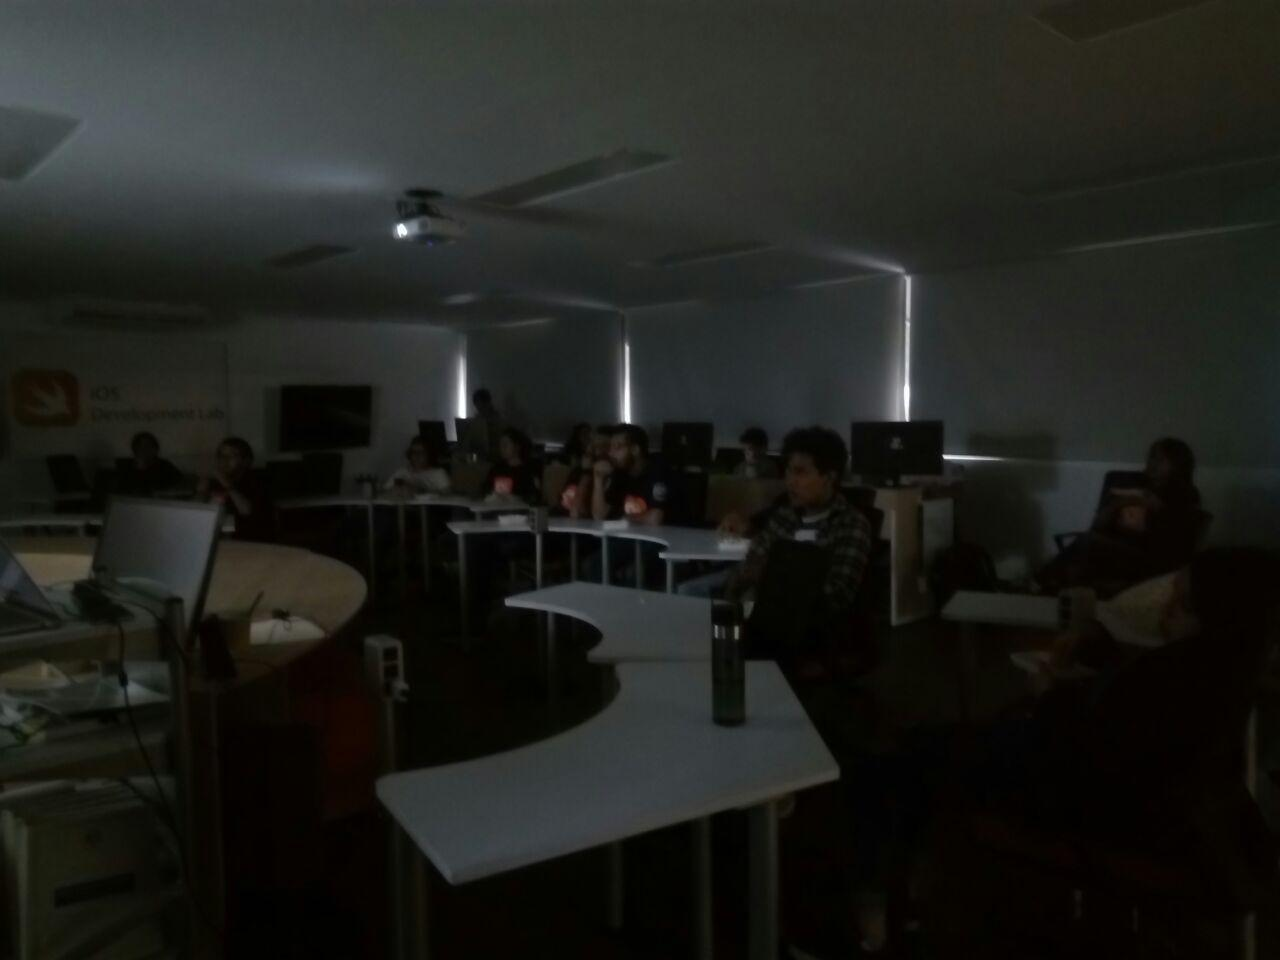
\includegraphics[width=0.75\textwidth]{images/openmovies-01}
      \caption{Asistencia de Proyección de OpenMovies en iOS Lab.}
      \label{fig:openmovies-01}
    \end{center}
  \end{figure}
  
  \subsection{Installfest.}  
  En la feria se estuvo en el stand el tiempo que también se dedicó a esta actividad.\\ En el stand conseguimos hablarles sobre nuestra agrupación a $\approx 200$ personas, aunado a esto, en el segundo día logramos obtener el correo de 20 estudiantes que están interesados en colaborar con nosotros.\\ Ayudamos en la instalación de GNU/Linux en 4 equipos y al stand llevamos una impresora 3D tal como se ve en la figura~\ref{fig:installfest-01}.
    \begin{figure}[H]
    \begin{center}
      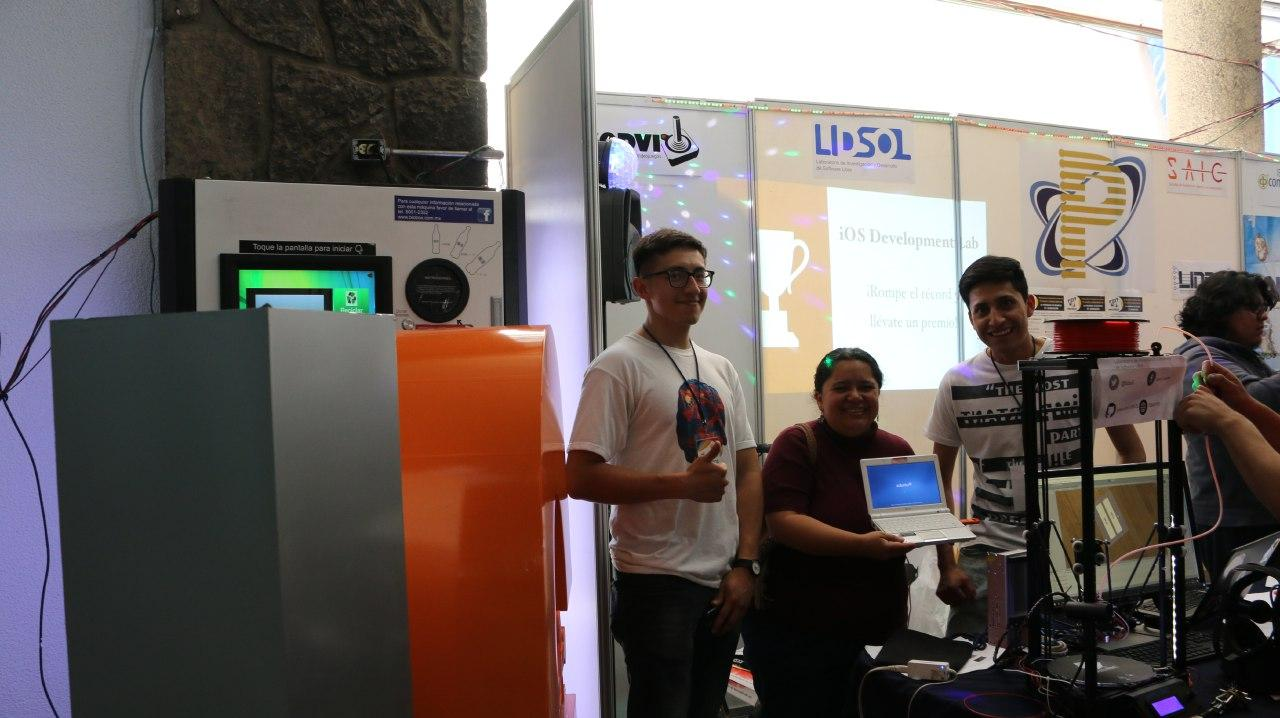
\includegraphics[width=0.75\textwidth]{images/installfest-01}
      \caption{Stand de LIDSOL durante la feria, se observa la impresora 3D y la realización de una instalación.}
      \label{fig:installfest-01}
    \end{center}
  \end{figure}
  
  \subsection{Taller de OpenScad. \textit{OpenScad para diseño de módelos parametrizables 2D y 3D} .}
  
  El taller de OpenScad tuvo un total de 19 inscritos vía online, sin embargo tuvo una asistencia total de 8 personas.
       \begin{figure}[H]
    \begin{center}
      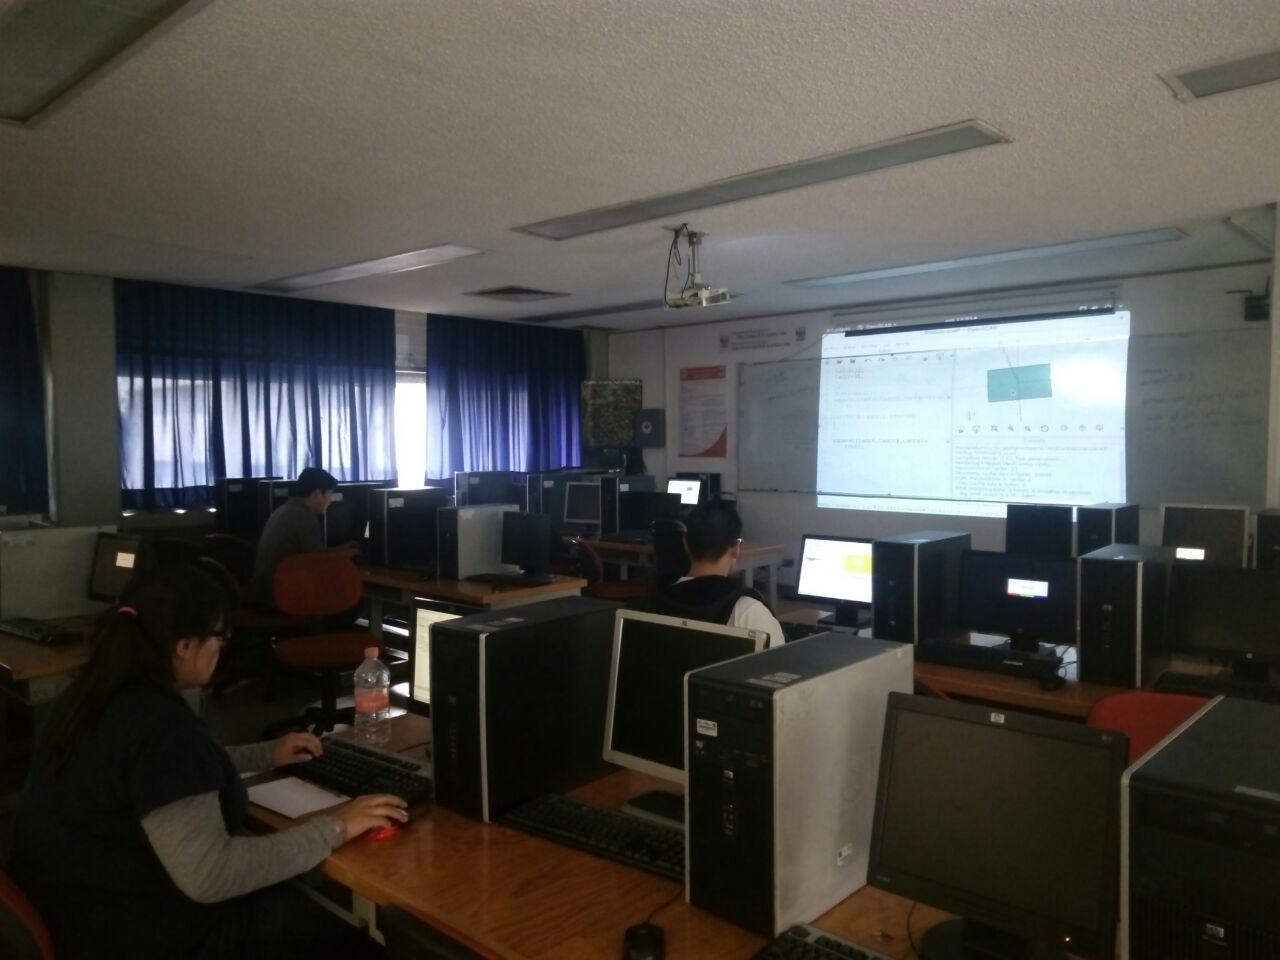
\includegraphics[width=0.75\textwidth]{images/openscad-01}
      \caption{Asistencia al taller de OpenScad el primer día.}
      \label{fig:openscad-01}
    \end{center}
  \end{figure}
  
  \subsection{Taller de monitoreo y administración de una impresora 3D. \textit{Administra tu impresora 3D en línea} .}   
  
El taller de de monitoreo y administración de una impresora 3D tuvo un total de 12 inscritos vía online y tuvo una asistencia total de 5 personas. Tal como se observa en la figura~\ref{fig:impresion-01}
       \begin{figure}[H]
    \begin{center}
      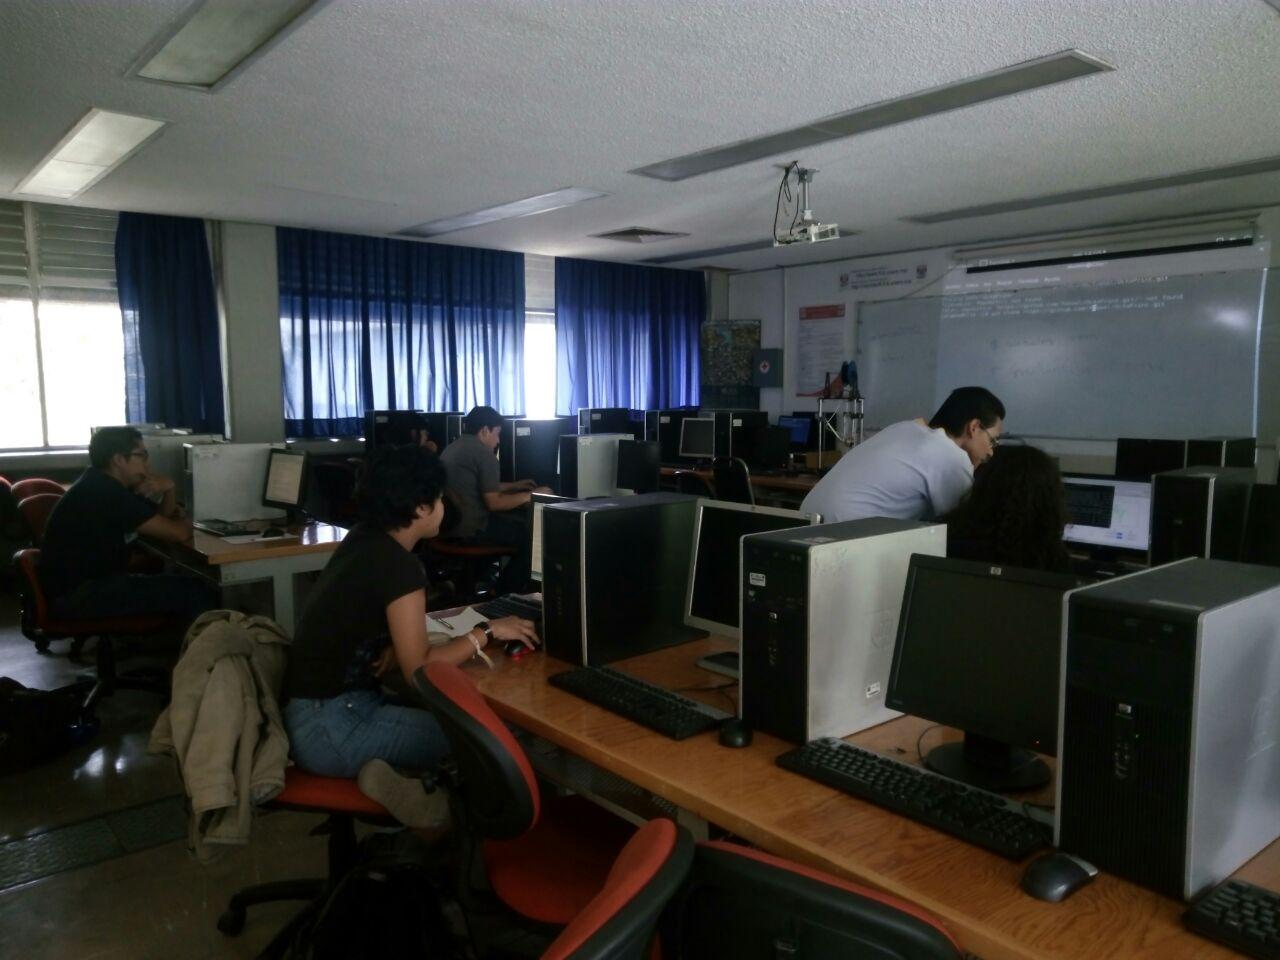
\includegraphics[width=0.75\textwidth]{images/impresion-01}
      \caption{Asistencia al taller de monitoreo y administración de una impresora 3D.}
      \label{fig:impresion-01}
    \end{center}
  \end{figure}
  
  \subsection{Taller de KiCad. \textit{ Tu primer PCB con KiCad} .}  
    El taller de KiCad tuvo un total de 20 inscritos vía online y tuvo una asistencia total de 14 personas.
       \begin{figure}[H]
    \begin{center}
      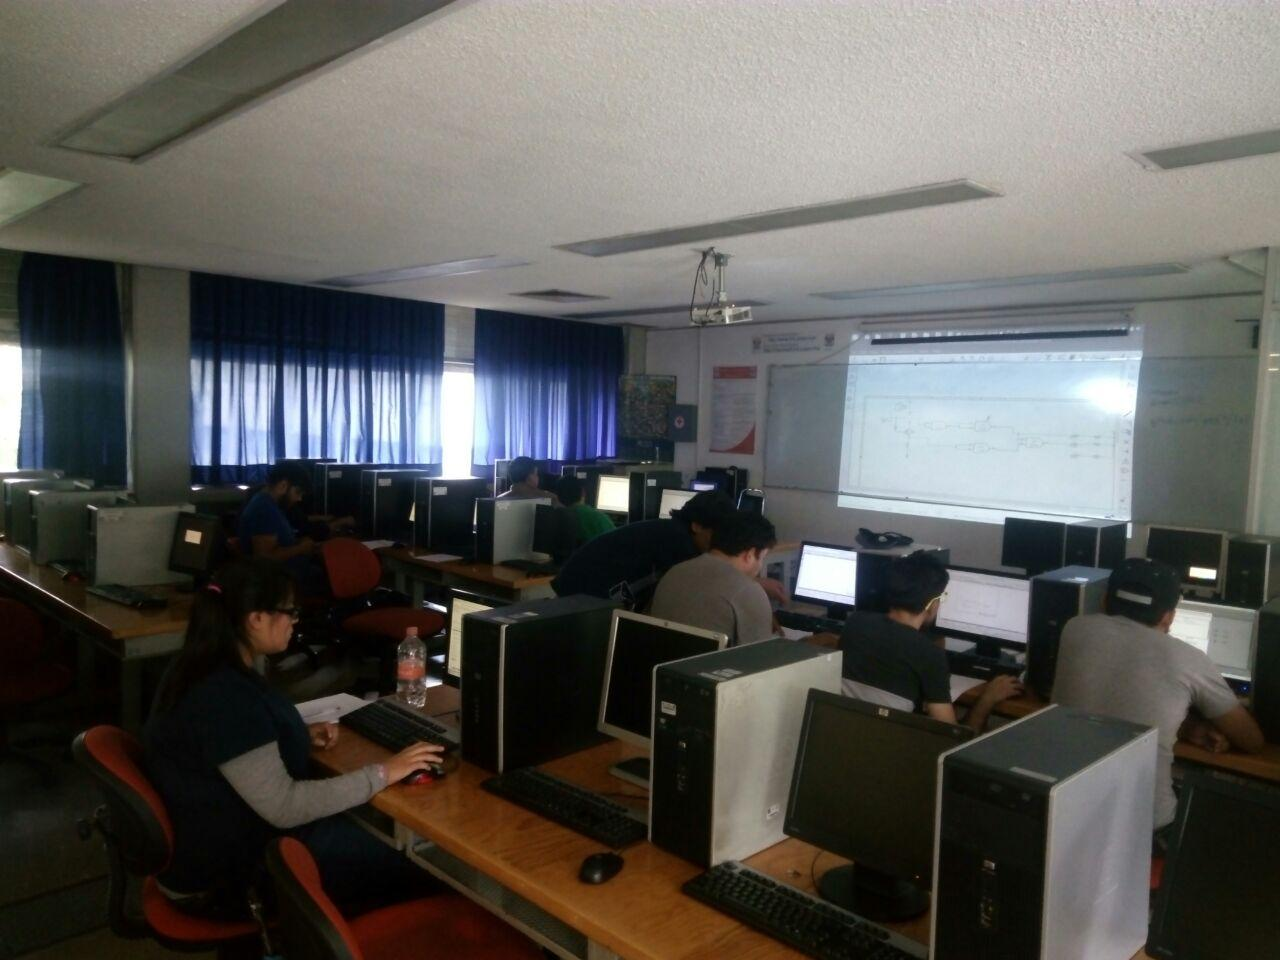
\includegraphics[width=0.75\textwidth]{images/kicad-01}
      \caption{Asistencia al taller de KiCad el primer día.}
      \label{fig:kicad-01}
    \end{center}
  \end{figure}   
  
  \begin{figure}[H]
    \begin{center}
      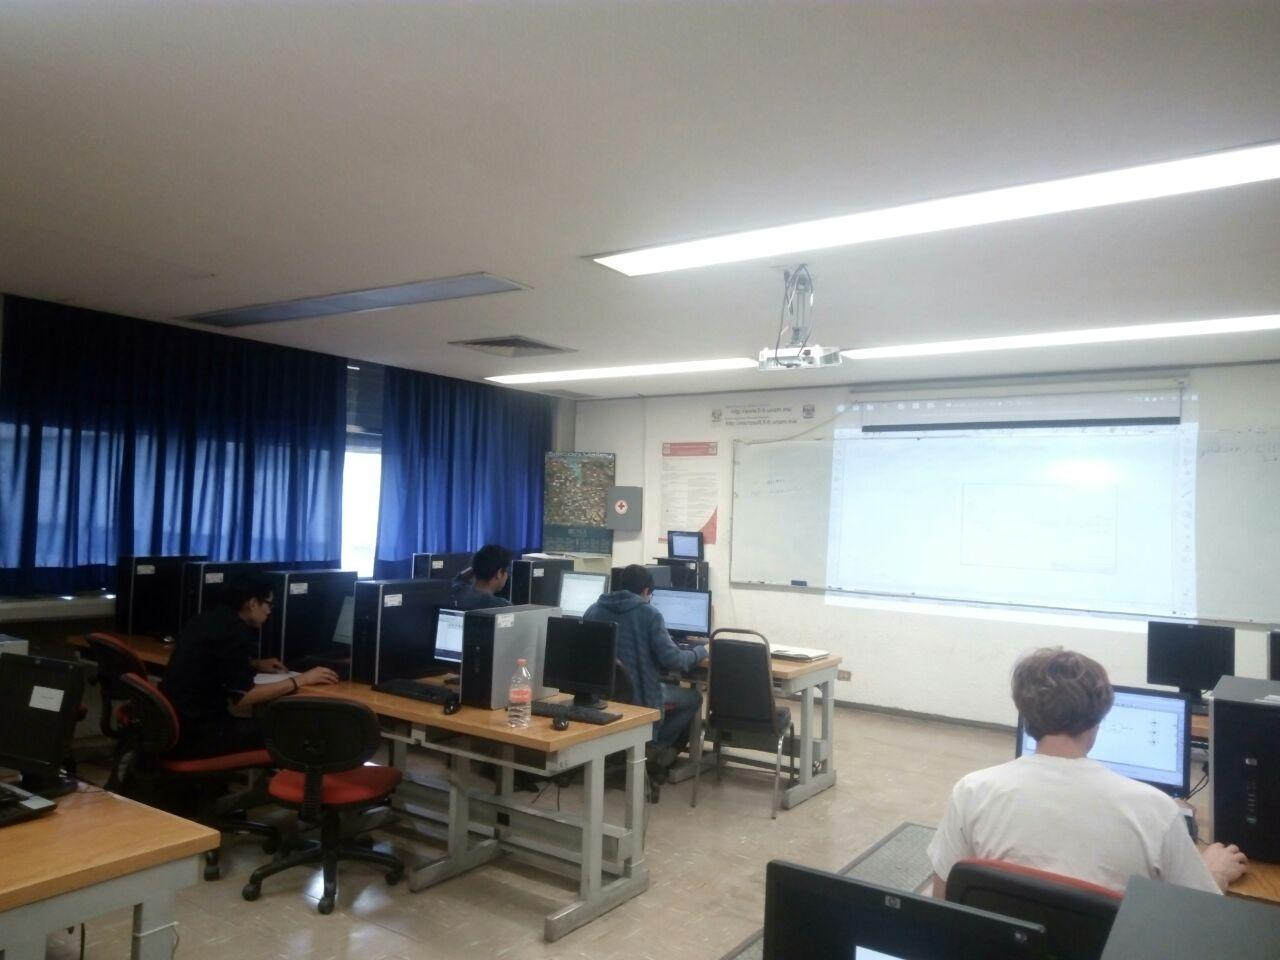
\includegraphics[width=0.75\textwidth]{images/kicad-02}
      \caption{Asistencia al taller de KiCad el segundo día.}
      \label{fig:kicad-02}
    \end{center}
  \end{figure}   
  
  \subsection{Taller de Nightly. \textit{Cómo contribuir a Firefox sin saber programación }.}  
  
El taller de  Nightly tuvo un total de 6 inscritos vía online y tuvo una asistencia.

       \begin{figure}[H]
    \begin{center}
      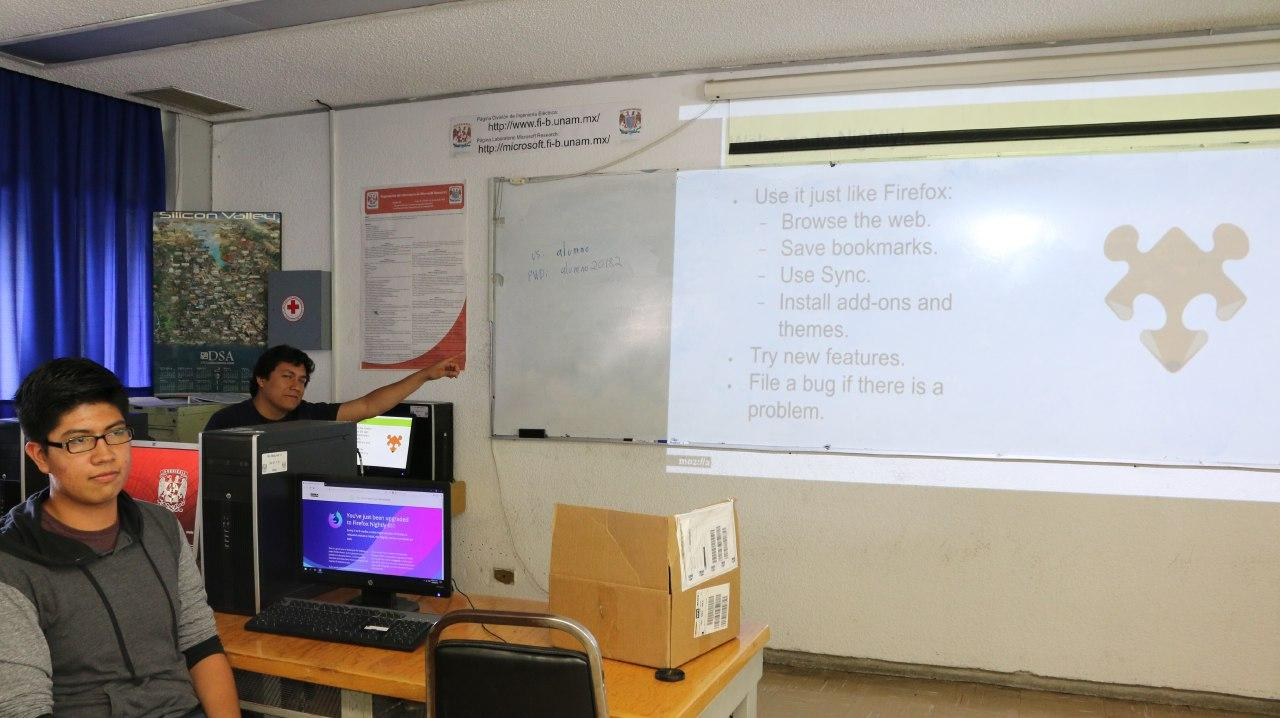
\includegraphics[width=0.75\textwidth]{images/nightly-01}
      \caption{Asistencia al taller de Nightly.}
      \label{fig:nightly-01}
    \end{center}
  \end{figure} 
  
  \subsection{Conferencia/Plática \textit{Privacidad, anonimato y derechos digitales} .}     
  En la conferencia, los asistentes se mostraron muy participativos y fueron alrededor de 80. Al final de la conferencia se les dio \textit{swag} de Tor.
             \begin{figure}[H]
    \begin{center}
      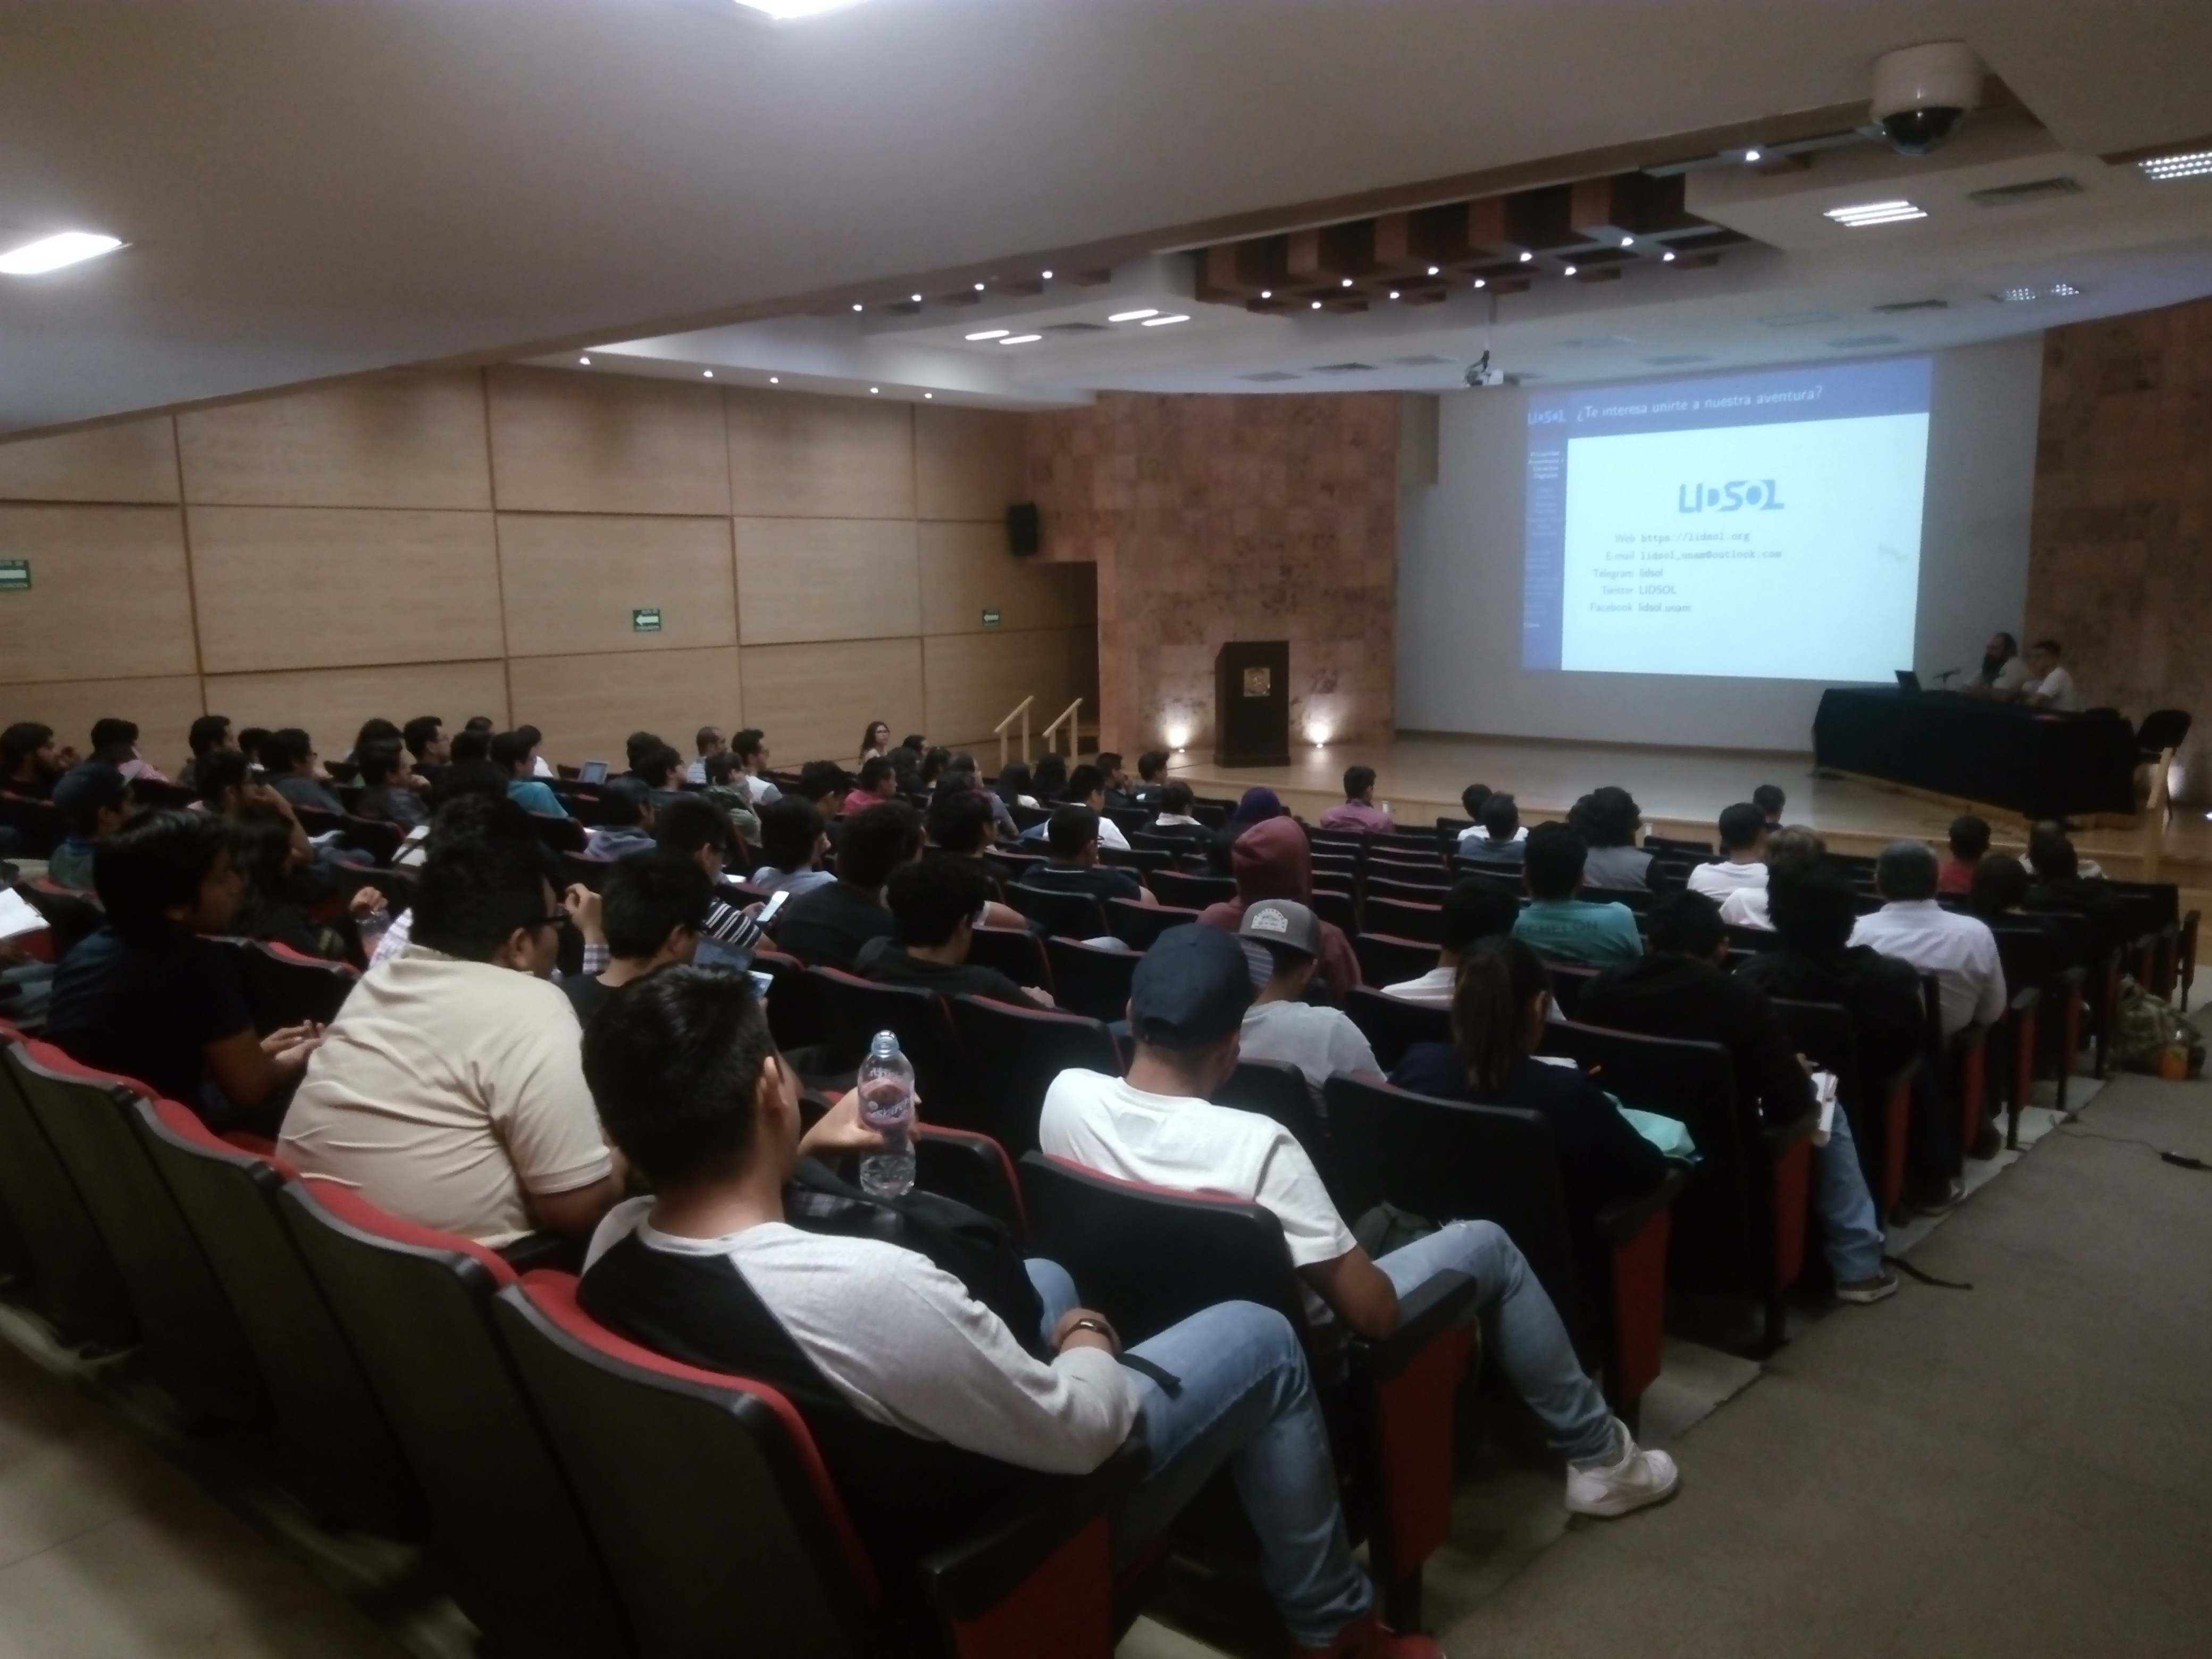
\includegraphics[width=0.375\textwidth]{images/tor-02}
      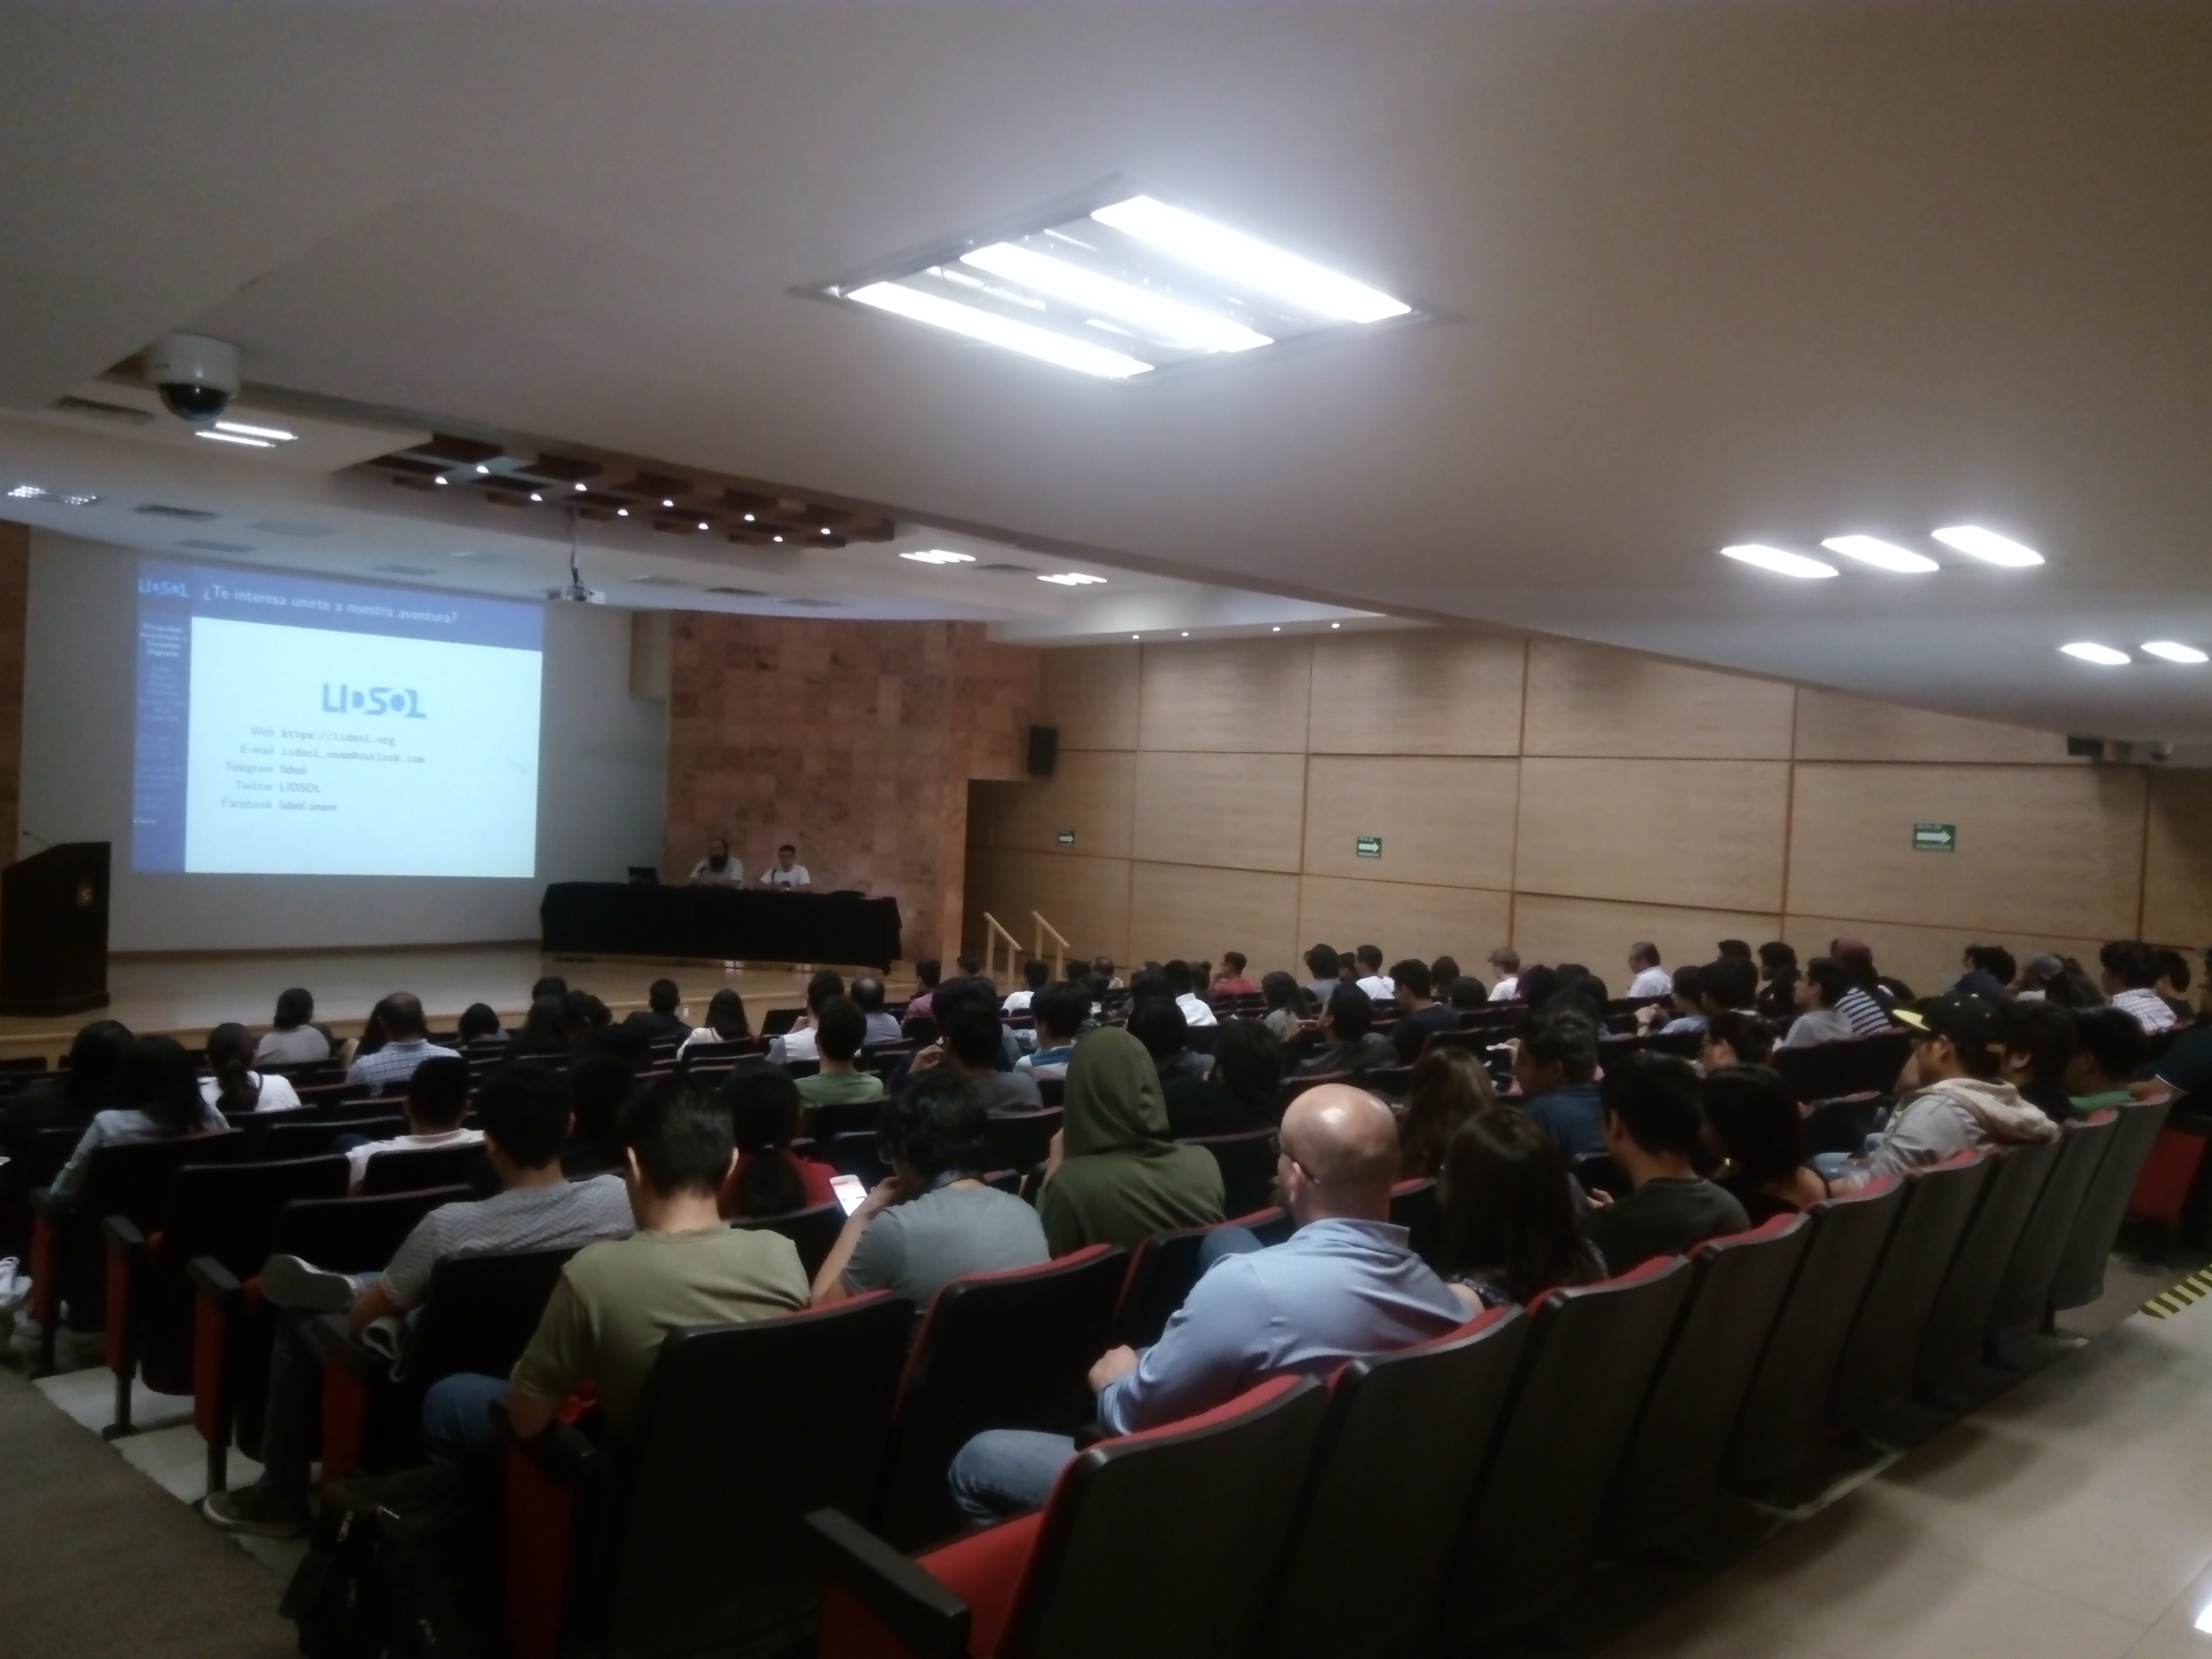
\includegraphics[width=0.375\textwidth]{images/tor-01}
      \caption{Asistencia a la conferencia  \textit{ Privacidad, anonimato y derechos digitales} .}
      \label{fig:tor}
    \end{center}
  \end{figure}  
  
  
  \subsection{Conferencia/Plática \textit{ ¿Hiciste cambios y ya no compila? Hablemos de Git} .} 
    En la conferencia, los asistentes se mostraron muy participativos y fueron alrededor de 50. Al final de la conferencia se les dio \textit{swag} de Github, mismo que no fue suficiente porque algunas personas se acercaron a pedirnos \textit{sheets}.
  
           \begin{figure}[H]
    \begin{center}
      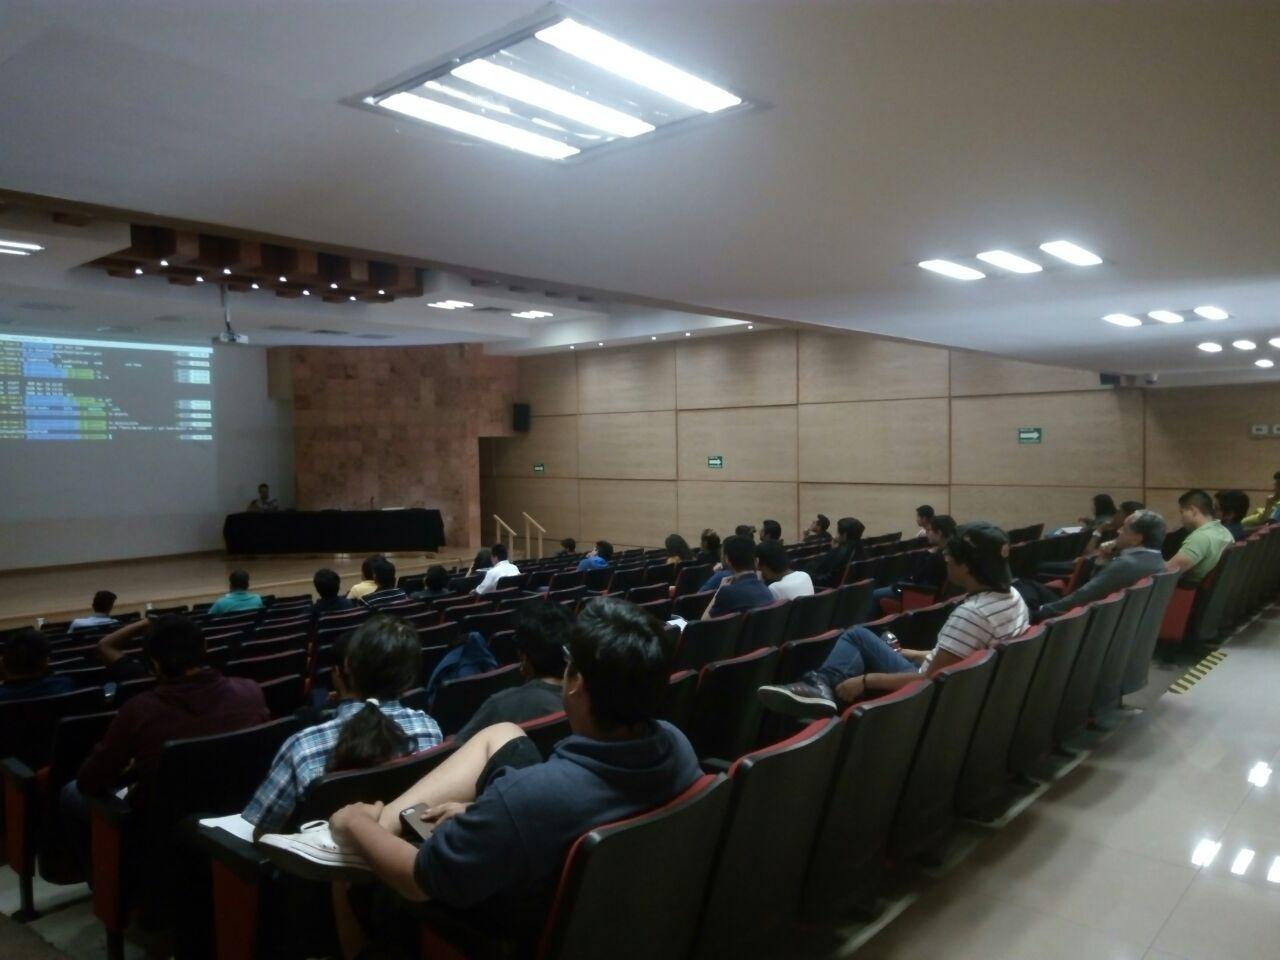
\includegraphics[width=0.375\textwidth]{images/git-02}
      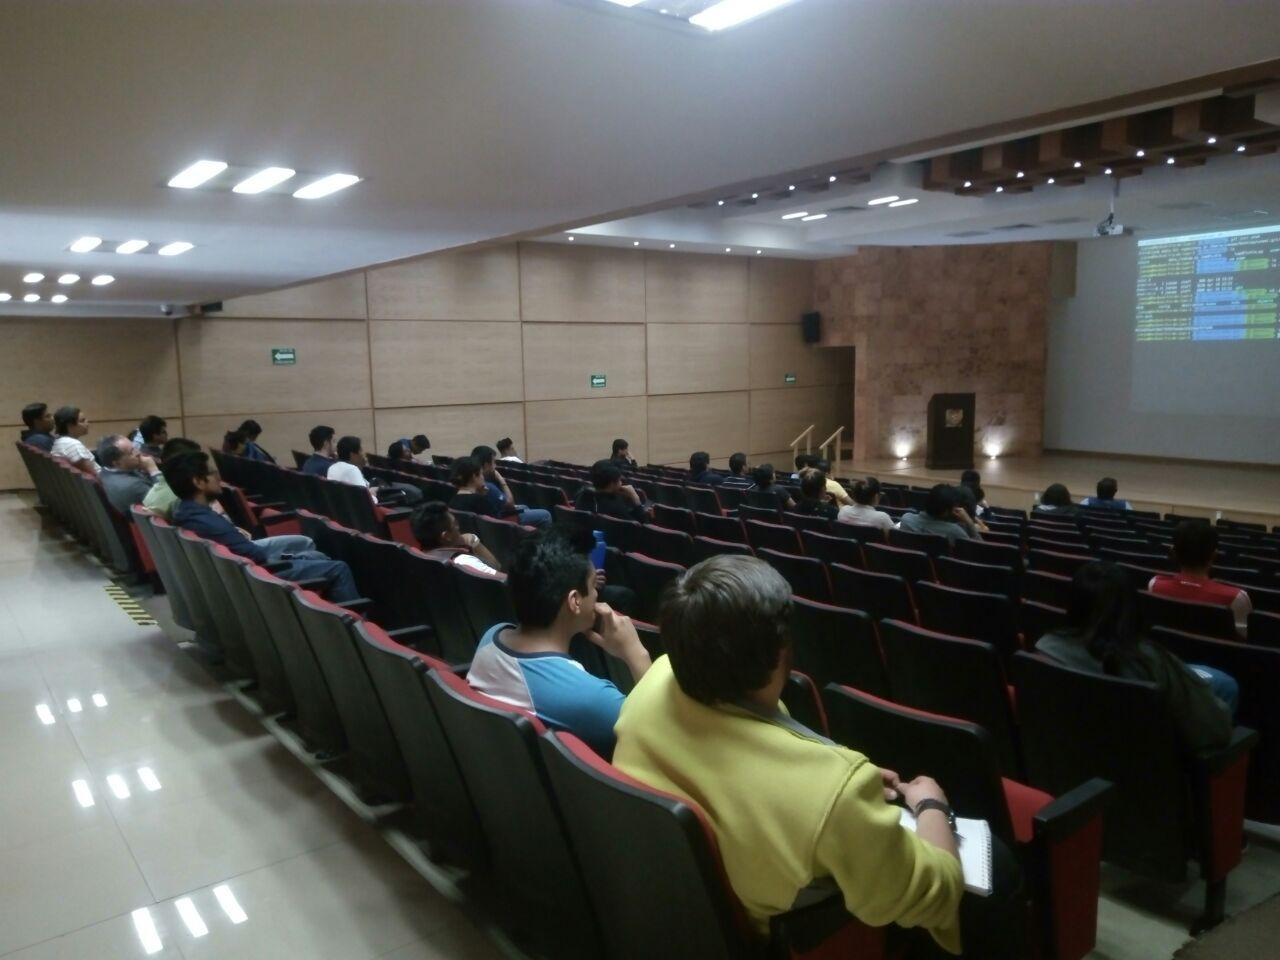
\includegraphics[width=0.375\textwidth]{images/git-03}
      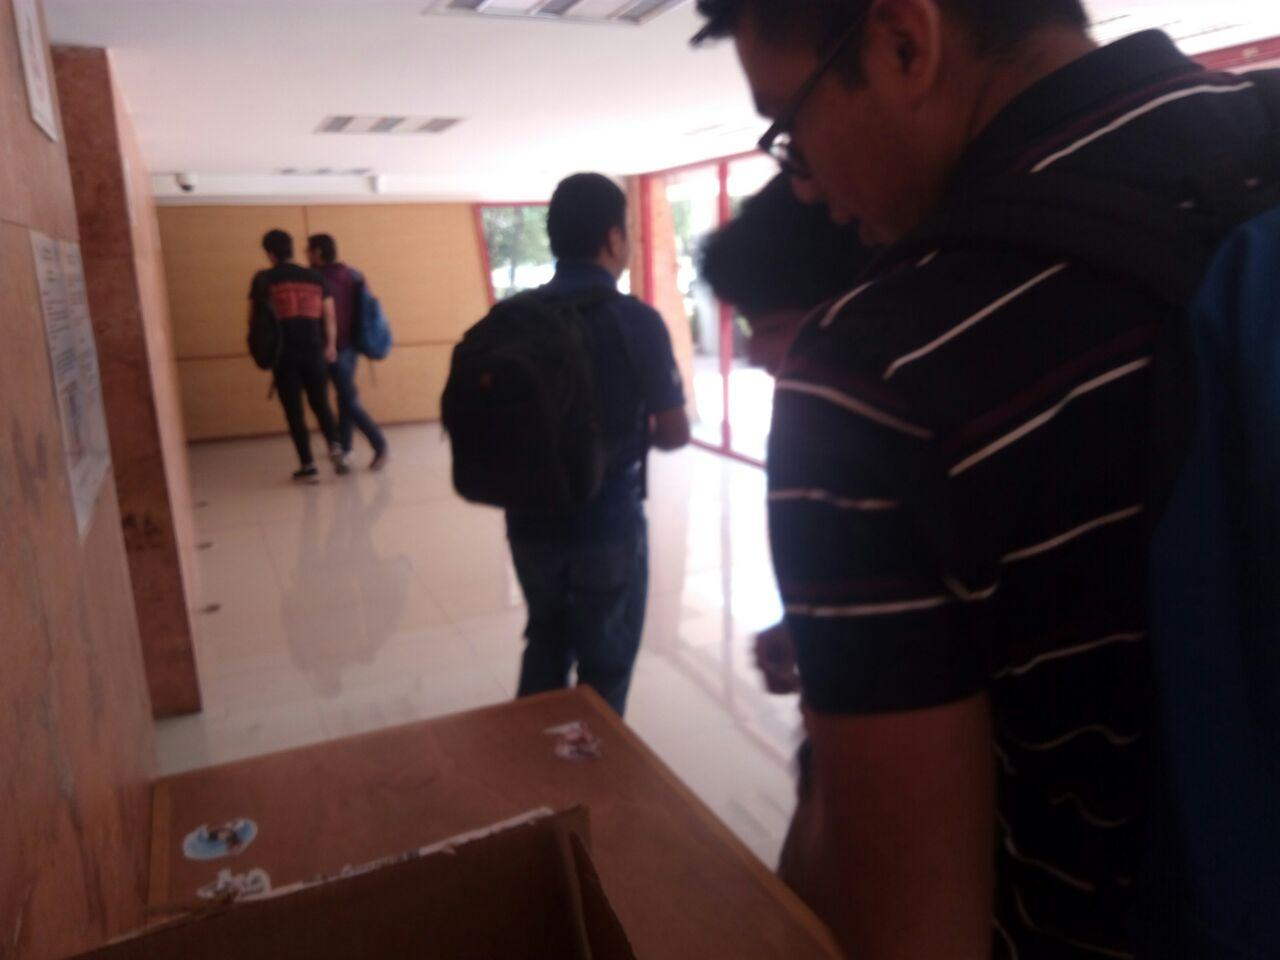
\includegraphics[width=0.375\textwidth]{images/git-01}
      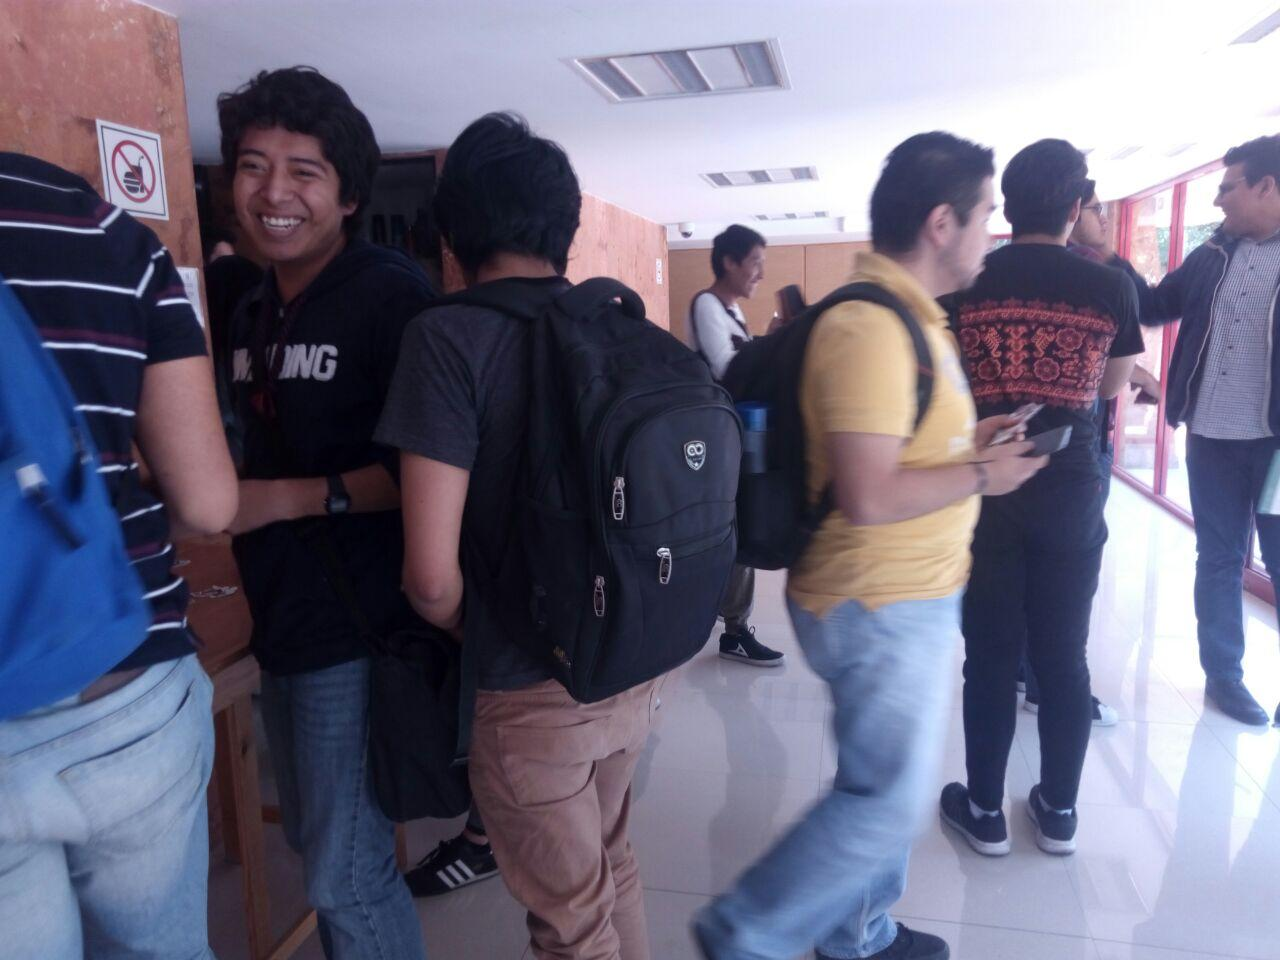
\includegraphics[width=0.375\textwidth]{images/git-04}
      \caption{Asistencia a la conferencia \textit{¿Hiciste cambios y ya no compila? Hablemos de Git}.}
      \label{fig:git}
    \end{center}
  \end{figure}  
  
  \subsection{Conferencia/Plática\textit{ No es tu amigo, es software privativo }.}  
       En la conferencia, los asistentes se mostraron muy participativos y fueron alrededor de 35. 
         \begin{figure}[H]
    \begin{center}
      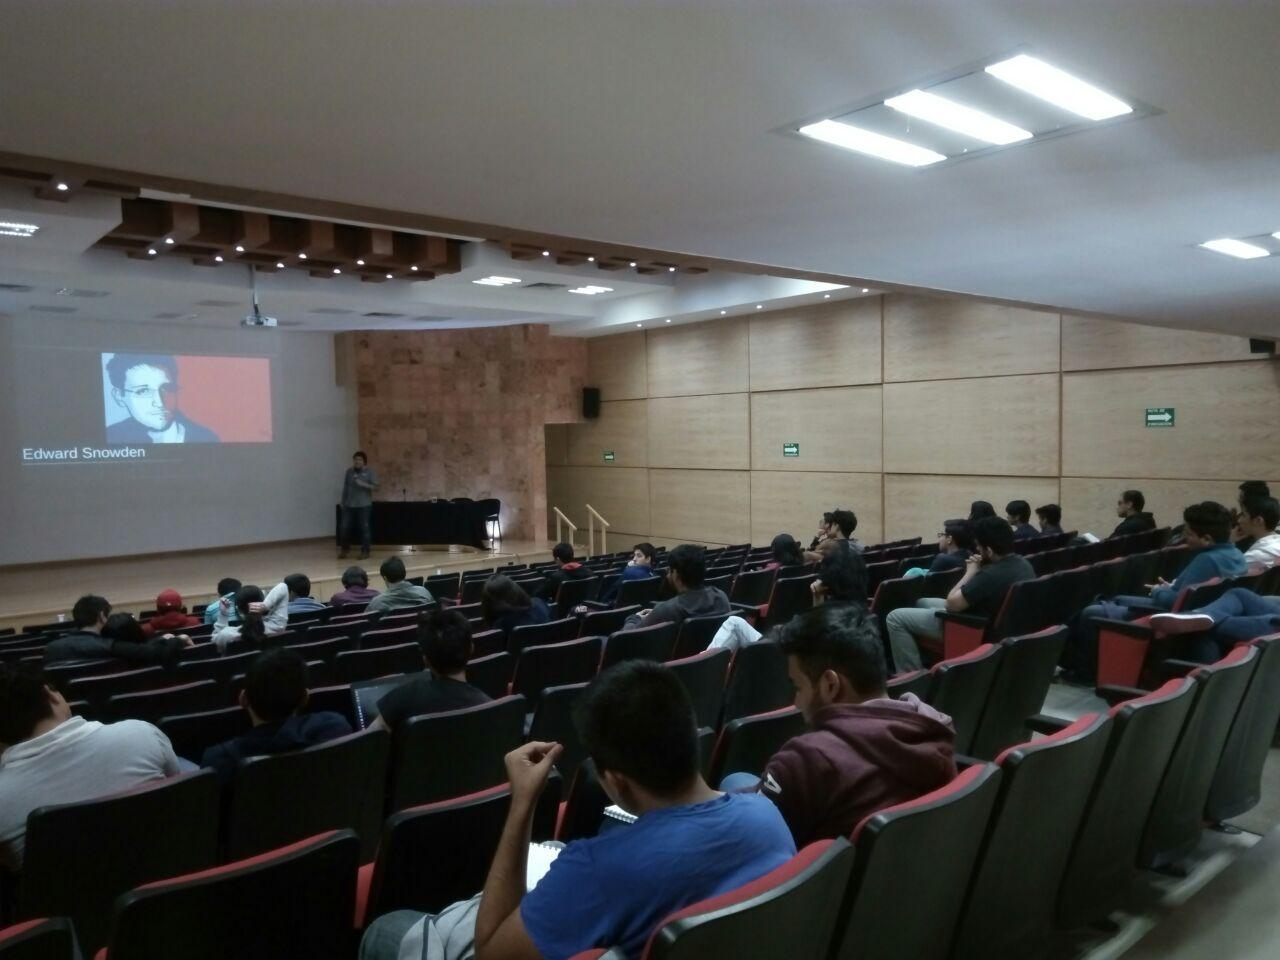
\includegraphics[width=0.75\textwidth]{images/privativo-01}
      \caption{Asistencia a la conferencia \textit{No es tu amigo, es software privativo} .}
      \label{fig:privativo-01}
    \end{center}
  \end{figure}  
  
  \newpage
  
       \section{Realimentación.}
  \subsection{General.}
  
    \begin{itemize}
    
    \item Consideramos que nuestra participación en la feria fue exitosa, y creemos que resulto así porque hubo una buena planeación y una participación activa y responsable de cada uno de los miembros que se comprometieron en las distintas actividades. \\Este resultado no habría sido posible sin el increíble equipo que hemos conformado alrededor de LIDSOL:
    \begin{itemize}
      \item Académicos que nos dieron su apoyo:
      \begin{itemize}
        \item Juan José Carreón Granados.
        \item Marduk Pérez, que nos vinculó con la DIE.
      \end{itemize}
      \item Miembros activos durante el evento:
          \begin{itemize}
      \item Nohemi Elvet
      \item Pablo Vivar
      \item Luis Vilchis
      \item Diego Barriga
      \item Emilio Cabrera
      \item Paul Aguilar
      \item Yesica Navarro
    \end{itemize}
    \item Conferencistas:
    \begin{itemize}
      \item Gunnar Wolf
      \item Pablo Flores
    \end{itemize}
      \item Asistentes que nos dieron su apoyo:
      \begin{itemize}
        \item Noemi Rodríguez
        \item Alexis Ríos
        \item Marisol Rios
        \item Luz Torres
        \item Gustavo Chávez 
      \end{itemize}
    \end{itemize}


    
    \item Mandamos un cartel por cada actividad, no sabiamos que había un límite de carteles por agrupación, lo que hizo que sólo pudieramos imprimir 5 carteles por actividad. En un futuro sería deseable que hicieramos un cartel que contuviera todas nuestras actividades.
    
    \item Los carteles se imprimieron tan solo 7 días hábiles antes de la feria, (y fuero pocos) por lo que no fue tan visible, creemos que si existiera un canal de comunicación más efectivo con la SSA esto no habría pasado, porque los carteles de nuestra parte estuvieron listos mucho antes.
    
    \item Existio conflicto del uso de la cámara, en futuros eventos sería deseable designar a una persona que se encargue de la cámara y documentar sea su única tarea durante ese evento.
    
    \item Nos dimos cuenta que al anunciar en los salones, hubo profesores que enviaron a sus alumnos por puntos extra, creemos que esos profesores formaron un pilar muy fuerte para que existiera asistencia en nuestras actividades. Es deseable que en futuros eventos podamos hablar con los profesores e imprimir una hoja con la información de las actividades para que sean ellos quienes inviten a los alumnos.
    
    \item El primer día no teniamos forma de enviar más información a las personas que se interesaban por LIDSOL en el stand, es importante crear un formato de registro para los interesados en futuros eventos.
    
    \item Debido a las conferencias, sacamos la lona de LIDSOL al auditorio para obtener visibilidad y tuvimos un incidente con la misma. Es regla no dejar las lonas en los auditorios, las lonas deben siempre devolverse a su lugar después de cada conferencia.
    
    \item Nos dimos cuenta que nos hace falta tener más material de apoyo llamativo y representativo de LIDSOL, porque sólo tenemos una lona y no ayudo mucho para visibilizar todas nuestras actividades (Conferencias en Auditorio Sotero Prieto, Stand en vestíbulo de Auditorio Javier Barros Sierra, Talleres
 en Anexo de Ineniería).
     
    \item Las conferencias del segundo día tuvieron mayor asistencia, y de hecho muchas personas preguntaron sobre la primera conferencia, no es bueno abrir el evento, pues las personas aún no están tan al tanto de las conferencias y pueden perderselas aunque les parezcan atractivas.
    
    \item Durante la feria la SSA entrega reconocimientos a las agrupaciones, sería recomendable tener a una sola persona encargada de recibir estos reconocimientos para que no se extravíen.
    
    \item La conexión con los ponentes siempre fue vía correo o mensajes privados de redes sociales, es importante pedirle al ponente su número celular para poder contáctarlo facilmente al momento de su conferencia.
    
    \item Nuestro desempeño en números:
    
    \begin{itemize}
    \item Alcance.
    \begin{itemize}
     \item En redes sociales nuestras actividades tuvieron 7200 visualizaciones.
      \item En total en los salones hicimos llegar el mensaje a aproximadamente 1400 alumnos.
      \hrulefill
      \item Tuvimos un alcance total de 8600 personas.
    \end{itemize}
    \item Involucrados.
    \begin{itemize}
      \item Durante la feria hubo un total de 438 personas que se involucraron, ya sea inscribiendose en talleres, pidiendo informes en el stand, asistiendo a las conferencias o pidiendo ayuda para instalación de GNU/Linux en sus equipos.
      \item Esto significa que aunque nuestras actividades llegaron a 8600 personas, sólo el 5.09\% de ellas decidieron participar en nuestras actividades, creemos que una forma de llegar al otro 94.91\% es con ayuda de los profesores como mencionamos en un punto anterior.
      \item De los involucrados, se llegó al 45.66\% a través del stand, el 37.67\% asistieron a las conferencias y el 13.01\% se inscribió a algún taller. Podemos ver entonces que el stand fue la actividad con mejor índice de involucrados, por lo tanto, si nuestras conferencias fueran cerca del stand, la asistencia a nuestras conferencias sería mucho mayor, porque los alumnos podrían ser enviados desde el stand hasta el auditorio Javier Barros Sierra, en lugar de hasta el Sotero Prieto.
    \end{itemize}
    \item Participantes.
    \begin{itemize}
      \item A pesar de que los estudiantes se involucraron en nuestras actividades (por ejemplo inscribiendose a los talleres o pidiendo informes en el stand) sólo 229, que representan el 52.28\%, participaron activamente en nuestras actividades (asistiendo a los talleres o conferencias) creemos que la forma de mejorar la participación de los involucrados es, por ejemplo, enviar correos de recordatorio o confirmación a los inscritos en los talleres. 
    \end{itemize}
    \end{itemize} 

  \end{itemize}
  
  \subsection{Proyección de OpenMovies.} 
  
  \begin{itemize}
    \item Aunque las personas mostraron interés en esta actividad, la palabra que utilizamos para llamar a esta actividad \texttt{OpenMovies} no transmitia nada en el contexto de la facultad, lo que provocó que al final esta actividad no tuviera la asistencia esperada.
    
    \item Nuestro desempeño en números:
    
    \begin{itemize}
    \item Alcance.
    \begin{itemize}
      \item El alcance se considera el mismo para todas las actividades, 8600 personas.
    \end{itemize}

    \item Asistencia.
    \begin{itemize}
      \item A esta actividad sólo asistieron 12 personas, que representan el 0.14\% de personas a quienes llegó la información.
      \item Estas 12 personas también representan al 2.74\% de involucrados en nuestras actividades, siendo la tercera actividad junto con el taller de impresión 3D, con menor número de involucrados. 
    \end{itemize}
    \end{itemize} 
    
  \end{itemize}
  
  
  \subsection{Installfest.}  
  
   \begin{itemize}
    \item Esta actividad tenía designada una carpa detrás del stand, pero no se hizo ahí porque no era visible, al final se opto por realizar el installfest en el stand, por lo que para futuros eventos no debería considerarse un espacio/carpa aparte para la realización de esta actividad.
    \item Creemos que nos falto tematizar el espacio que estaba dedicado a esta actividad porque personas qe participaron comentaron que no nos encontraban, además al estar tematizado llamaría más la atención y exitiría una mayor participación.
    \item De nuestra parte nos falto tener las ISOs en al menos tres USBs listos para usarse, porque aunque teníamos muchas distros descargadas, los participantes tuvieron que esperar mucho para iniciar su instalación.
    \item En un principio consideramos los horarios de los miembros de LIDSOL para definir los horarios que estaríamos en stand y considerabamos hasta 7 u 8 de la noche. En la feria nos dimos cuenta que todos los stands se retiran a las 5 pm, por lo que en futuras ediciones deberiamos considerar nuestro horario en función de esto.
    
    
    \item Nuestro desempeño en números:
    
    \begin{itemize}
    \item Alcance.
    \begin{itemize}
      \item El alcance se considera el mismo para todas las actividades, 8600 personas.
    \end{itemize}

    \item Asistencia.
    \begin{itemize}
      \item A esta actividad sólo asistieron 5 personas, que representan el 0.05\% de personas a quienes llegó la información.
      \item Estas 5 personas también representan al 0.91\% de involucrados en nuestras actividades, siendo la actividad con menor índice de involucrados. Creemos que la participación en esta actividad puede mejorar en futuras ediciones si compartimos la información de esta actividad fuera de la facultad e incluso fuera de la universidad.
    \end{itemize}
    \end{itemize} 
    
  \end{itemize}
  \subsection{Taller de OpenScad. \textit{OpenScad para diseño de módelos parametrizables 2D y 3D} .}
  
  \begin{itemize}
    \item El desarrollo del curso fué satisfactorio porque se logró impartir conocimientos acerca del modelado parametrizable a través del entorno de desarrollo con OpenSCAD además de difundir sobre el uso de alternativas de software libre para desarrollo de prototipos en ingeniería.
    
    \item Se dió a conocer también sobre el proyecto del repositorio sobre códigos libres parametrizables de la organización LIDSOL en GitHub.
    
    %Aquí van comentarios de Pabs.
    
    \item Nuestro desempeño en números:
    
    \begin{itemize}

    
    \item Inscritos.
    \begin{itemize}
      \item Se registraron 19 alumnos vía online.
      \item Estos 19 alumnos representan al 4.34\% de involucrados en nuestras actividades, siendo la sexta actividad con mayor número de involucrados. 
    \end{itemize}
    
    \item Asistencia.
    \begin{itemize}
      \item Hubo 8 asistentes que representan el 42.11\% de los inscritos para esta actividad, lo que significa que tiene el segundo lugar con mejor asistencia de los talleres impartidos. 
    \end{itemize}
    \end{itemize} 
    
  \end{itemize}
  
  
  \subsection{Taller de monitoreo y administración de una impresora 3D. \textit{Administra tu impresora 3D en línea} .}  
  
    \begin{itemize}
    \item Creemos que la asistencia fue baja porque muy pocas personas tienen impresoras 3D, por lo que sería mejor hacer un estudio de las personas que tienen impresoras 3D en la facultad, para decidir si volvemos a hacer talleres de este tipo.
    \item Aunque no hubo la asistencia esperada, el taller resultó muy útil a los asistentes, que después regresaron a LIDSOL para aprender más.
    
    \item Nuestro desempeño en números:
    
    \begin{itemize}

    
    \item Inscritos.
    \begin{itemize}
      \item Se registraron 12 alumnos vía online.
      \item Estos 12 alumnos representan al 2.74\% de involucrados en nuestras actividades, siendo la tercera actividad junto con la proyección de OpenMovies con menor número de involucrados. 
    \end{itemize}
    
    \item Asistencia.
    \begin{itemize}
      \item Hubo 5 asistentes representan el 41.67\% de los inscritos para esta actividad, lo que significa que tiene el tercer lugar con mejor asistencia de los talleres impartidos. 
    \end{itemize}
    \end{itemize} 
    
  \end{itemize}  
  \subsection{Taller de KiCad.  \textit{Tu primer PCB con KiCad} .}  
  
  
    \begin{itemize}
    \item Durante el primer día me di cuenta de la dificultad de guiar a muchas personas en el uso de un software si no se les dice explicitamente que se debe hacer, el segundo día corregí este error.
    \item Me parece que los participantes se llevaron una herramienta (un checklist) que les ayudó mucho a que el taller se manejara de manera dinámica.
    \item Reitero, una forma de atraer más alumnos es informar a los profesores sobre los talleres, sobretodo aquellos en cuya materia le puedan dar uso a lo aprendido en el taller.
    
    \item Nuestro desempeño en números:
    
    \begin{itemize}
 
    
    \item Inscritos.
    \begin{itemize}
      \item Se registraron 20 alumnos vía online.
      \item Estos 20 alumnos representan al 4.54\% de involucrados en nuestras actividades, siendo la quinta actividad con mayor número de involucrados. 
    \end{itemize}
    
    \item Asistencia.
    \begin{itemize}
      \item Hubo 14 asistentes representan el 70.00\% de los inscritos para esta actividad, lo que significa que tiene el primer lugar con mejor asistencia de los talleres impartidos. 
    \end{itemize}
    \end{itemize} 
    
  \end{itemize}     
  \subsection{Taller de Nightly. \textit{Cómo contribuir a Firefox sin saber programación }.}  
  
   
    \begin{itemize}
    \item Este taller no tuvo el impacto que se esperaba, creemos que una manera de mejorar esto es apoyarse en la comunidad de Mozilla para tener ayuda con la difusión.
    
    \item Nuestro desempeño en números:
    
    \begin{itemize}
 
    
    \item Inscritos.
    \begin{itemize}
      \item Se registraron 6 alumnos vía online.
      \item Estos 6 alumnos representan al 1.37\% de involucrados en nuestras actividades, siendo la segunda actividad con menor número de involucrados. 
    \end{itemize}
    
    \item Asistencia.
    \begin{itemize}
      \item Hubo un asistente que representa al 16.67\% de los inscritos para esta actividad, lo que significa que tiene el primer lugar con menor asistencia de los talleres impartidos. 
    \end{itemize}
    \end{itemize} 
    
  \end{itemize}  
  
  \subsection{Conferencia/Plática \textit{Privacidad, anonimato y derechos digitales }.}     
  
  \begin{itemize}
    \item Esta fue la última conferencia y fue la que tuvo mejor asistencia, creemos que entre los factores principales de esto, están que visitamos la facultad de politicas para que se distribuyera la información y pedimos a un profesor que nos llevara a su grupo, además uno de los ponentes es muy reconocido.
    
    \item Nuestro desempeño en números:
    
    \begin{itemize}
    \item Alcance.
    \begin{itemize}
      \item El alcance se considera el mismo para todas las actividades, 8600 personas.
    \end{itemize}

    \item Asistencia.
    \begin{itemize}
      \item A esta actividad asistieron 80 personas, que representan el 0.93\% de personas a quienes llegó la información.
      \item Estas 80 personas también representan al 18.26\% (casi una quinta parte) de involucrados en nuestras actividades, siendo la actividad con el segundo mejor índice de involucrados. 
    \end{itemize}
    \end{itemize} 
    
  \end{itemize}
  
  \subsection{Conferencia/Plática \textit{¿Hiciste cambios y ya no compila? Hablemos de Git}.} 
  
    \begin{itemize}
    \item Esta fue la segunda conferencia y teniamos \textit{swag} para entregar, en algún punto nos descuidamos y los asistentes revisaron las cosas del \textit{staff} con tal de encontrar más calcamonías, aprendimos que no debe dejarse al alcance de los asistentes sin supervisión las cosas del \textit{staff} porque pueden llegar a ser invasivos.
    \item Esta actividad también tuvo buena asistencia porque un profesor llevó a su grupo y tomo lista al final de la conferencia, se reitera, los profesores son pieza clave para que exista participación de los alumnos.
    
    \item Nuestro desempeño en números:
    
    \begin{itemize}
    \item Alcance.
    \begin{itemize}
      \item El alcance se considera el mismo para todas las actividades, 8600 personas.
    \end{itemize}

    \item Asistencia.
    \begin{itemize}
      \item A esta actividad asistieron 50 personas, que representan el 0.58\% de personas a quienes llegó la información.
      \item Estas 50 personas también representan al 11.42\%  de involucrados en nuestras actividades, siendo la actividad con el tercer mejor índice de involucrados. 
    \end{itemize}
    \end{itemize} 
    
  \end{itemize}
  \subsection{Conferencia/Plática  \textit{No es tu amigo, es software privativo} .}  
  
      \begin{itemize}
    \item Esta conferencia al ser la primera tuvo muy baja asistencia, pero existio un buen recibimiento e interés de la misma, en futuras ediciones seria conveniente no elegir nuestras conferencias al principio del evento.
    
    \item Nuestro desempeño en números:
    
    \begin{itemize}
    \item Alcance.
    \begin{itemize}
      \item El alcance se considera el mismo para todas las actividades, 8600 personas.
    \end{itemize}

    \item Asistencia.
    \begin{itemize}
      \item A esta actividad asistieron 35 personas, que representan el 0.41\% de personas a quienes llegó la información.
      \item Estas 35 personas también representan al 7.99\%  de involucrados en nuestras actividades, siendo la actividad con el cuarto mejor índice de involucrados. 
    \end{itemize}
    \end{itemize} 
    
  \end{itemize}
   
%%%%%%%%%%%%%%%%%%%%%%%%%%%%%%%%%%%%%%%%%%%%%%%%%%%%%%%%%%%%%%%%%%%%%%%%%%%%%%%%%%%%%%%%%
  


%%%%%%%%%%%%%%%%%%%%%%%%%%%%%%%%%%%%%%%%%%%%%%%%%%%%%%%%%%%%%%%%%%%%%%%%%%%%%%%%%%%%%%%%%

\end{document}
